\documentclass[10pt,twocolumn,letterpaper,french]{article}

\usepackage[utf8]{inputenc} 

\usepackage{cvpr}
\usepackage{times}
\usepackage{epsfig}
\usepackage{graphicx}
\usepackage{amsmath}
\usepackage{amssymb}
\usepackage[francais]{babel}
\usepackage{amsmath}
\newcommand\norm[1]{\left\lVert#1\right\rVert}
\usepackage[ruled,vlined]{algorithm2e}
\usepackage{mathrsfs}
\usepackage[toc,page]{appendix}
\usepackage[margin=0.6in]{geometry}
\usepackage[export]{adjustbox}
\usepackage{placeins}

%\pagenumbering{alph}


%\pagenumbering{gobble}

% Include other packages here, before hyperref.

% If you comment hyperref and then uncomment it, you should delete
% egpaper.aux before re-running latex.  (Or just hit 'q' on the first latex
% run, let it finish, and you should be clear).
\usepackage[breaklinks=true,bookmarks=false]{hyperref}

\cvprfinalcopy % *** Uncomment this line for the final submission

\def\cvprPaperID{****} % *** Enter the CVPR Paper ID here
\def\httilde{\mbox{\tt\raisebox{-.5ex}{\symbol{126}}}}

% Pages are numbered in submission mode, and unnumbered in camera-ready
%\ifcvprfinal\pagestyle{empty}\fi
\setcounter{page}{1}
\begin{document}

%%%%%%%%% TITLE
\title{Amélioration du noyau des systèmes siamois\\pour le suivi d'objets}

\author{Paulin Brissonneau\\
CentraleSupélec\\
{\tt\small paulin.brissonneau@student-cs.fr}}
% For a paper whose authors are all at the same institution,
% omit the following lines up until the closing ``}''.
% Additional authors and addresses can be added with ``\and'',
% just like the second author.
% To save space, use either the email address or home page, not both^



\maketitle
%\thispagestyle{empty}

%%%%%%%%% ABSTRACT
\begin{abstract}

Les avancées récentes en suivi d'objet dans les vidéos tirent leurs profits de métriques de similitude approximées par des réseaux de neurones profonds. On s'intéresse en particulier au siamFC \cite{siamfc}, méthode à base de réseaux siamois qui utilise des extracteurs de caractérisitiques pour comparer, à chaque instant de la vidéo, l'image la cible à suivre et l'image de recherche. Dans sa forme originale, le siamFC utilise une architecture de type AlexNet à cinq couches ainsi que une seule et unique image de la cible fournie avant le début du suivi qu'il cherche ensuite dans chaque image de la séquence vidéo. Dans ce rapport, nous montrons que l'architecture de référence du siamFC peut-être légèrement améliorée, puis nous montrons qu'il est aussi possible d'améliorer les performances du suiveur d'objet en prenant en compte, dans les bonnes proportions, un historique glissant des apparences de l'objet à suivre.

\end{abstract}

%%%%%%%%% BODY TEXT
\section*{Introduction}

Le suivi d'objets est un domaine de la vision numérique qui consiste à suivre un ou plusieurs objets présents sur une vidéo.
   Pendant longtemps, l'état de l'art était tenu par des algorithmes purement statistiques, qui associaient des probabilités de correspondance entre les formes présentes sur deux images à la suite dans une vidéo. Depuis quelques années, le domaine du suivi d'objets a été drastiquement influencé par le développement de l'apprentissage profond. En quelques années, les algorithmes basés sur des métriques profondes ont détrôné tous les algorithmes classiques à l'état de l'art. L'utilisation de réseaux profonds permet une comparaison plus fine des différents objets et résiste mieux aux occlusions de longue durée grâce à une comparaison des objets à un haut niveau d'abstraction. \\
   
   L'introduction des réseaux profonds en suivi d'objets prend plusieurs formes. Les méthodes basées sur les détections (\textit{two stages trackers}) infèrent le suivi en deux étapes distinctes : d'abord une détection des objets présents sur l'image, puis une association des différents objets d'une image à la suivante. Cette façon de faire donne des résultats remarquables pour un temps de calcul des inférences court. Les algorithmes SORT \cite{SORT} puis sa variante \textit{à métrique profonde} deepSORT \cite{deepSORT} sont des représentants de cette famille.
   
   Au contraire, les méthodes unifiées font toutes ces opérations en une seule étape. De nombreux travaux ont tenté d'unifier ces deux étages avec différentes méthodes. Parmi les solutions unifiées, celles basées sur les réseaux siamois se sont emparées de l'état de l'art et montrent des performances très prometteuses \cite{siamfc, siamfcplusplus, siamMask}. 
   
   Or, contrairement aux méthodes à détection, les méthodes à réseaux siamois dans leurs formes simples se contentent de chercher l'image initiale de la cible dans chacune des images de la vidéo. Ceci ne permet pas d'utiliser l'information relative à l'historique de l'apparance de la cible dans la séquence vidéo, comme le font structurellement les méthodes à détection. Cette absence d'historique a des avantages, notamment le fait de pouvoir suivre une cible sur des fragements de vidéos voire des images indépendantes. Cela apporte aussi des inconvénients, comme une moins bonne résistance aux changements d'apparence, et un risque accru de confusion entre plusieurs instances semblables d'un même objet dans une vidéo.
   
   C'est pour cette raison qu'il est intéressant d'étudier l'interêt d'un système de stockage en mémoire des images de la cible tout au long de la séquence vidéo. Dans ce rapport, nous introduisons l'aspect de mémorisation en utilisant un \textit{noyau glissant}, c'est-à-dire en gardant un historique des cartes de caractéristiques profondes extraites de la cible.\\
  
  Nous étudions les comportements des systèmes siamois en général et ne cherchons pas à atteindre les performances de l'état de l'art. C'est pour cette raison que nous utiliserons l'architecture simple du siamFC \cite{siamfc}, et non des architectures plus récentes et plus poussées qui présentent de meilleurs résultats. Grâce à une architecture de référence sobre, nous serons plus à même d'étudier en détail l'effet de nos modifications et d'interpréter nos résultats sans autres effets parasites que pourraient apporter des architectures complexes.

\section*{État de l'art}

\subsubsection*{Réseaux Siamois}

Les réseaux siamois sont une ancienne idée qui a fait son apparition en 1994 grâce à Bromley et al. \cite{siamese}. Le principe des réseaux siamois est d'encoder de manière non-linéaire deux entrées différentes avec un même réseau extracteur de caractéristiques. L'objectif est que les cartes de caractéristiques obtenues soient porteuses de suffisamment d'information sémantique pour pouvoir comparer les données initialement données en entrée. À titre d'exemple, pour comparer deux visages et dire si ils appartiennent à la même personne, on encode chacun des deux visages par un seul et même réseaux, la comparaison des cartes de caractéristiques nous donnera une idée de la similarité des deux visages, non pas d'un point de vu photographique, mais d'un point de vue sémantique. \\

\begin{figure}[!h]
\centering
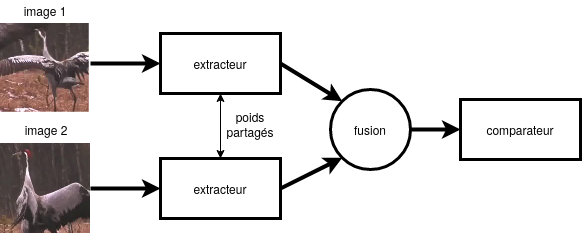
\includegraphics[width=260pt]{images/principe/siamese.png}
\caption{\textbf{Structure générale des réseaux siamois.}}
\label{siamese}
\end{figure}

Les réseaux siamois sont donc constitués de principalement deux étages, plus ou moins séparés selon les applications. La structure globale d'un réseau siamois est explicité sur la figure \ref{siamese}. Le premier étage est l'extracteur de caractéristiques qui sera le plus souvent, lorsque les données sont structurées et compositionnelles, un réseau convolutionnel. Le deuxième étage permet la comparaison des caractéristiques extraites peut prendre plusieurs formes, allant de la simple distance vectorielle au réseau de neurones. Il y a parfois un étage intermédiaire permettant de fusionner les cartes de caractéristiques. Il peut s'agir par exemple d'une simple soustraction termes à termes ou d'une corrélation croisée (\textit{cross-correlation}).\\


Les réseaux siamois ont été utilisés pour un très grand nombre de tâches, à savoir le \textit{hashing} \cite{hashing}, le \textit{clustering} \cite{clustering} et surtout l'apprentissage sur peu d'exemples (\textit{few-shot learning}) \cite{one-shot}. De par leur structure, ils sont aussi particulièrement adaptés à la comparaison de deux données, comme par exemple la vérification faciale \cite{face_verif}, la localisation \cite{tompson2015efficient}, la rénovation d'images \cite{gordo2017endtoend}, et bien sûr le suivi d'objets \cite{siamfc, siamfcplusplus, siamMask, trackRCNN}.

\subsubsection*{Suivi d'objets}

\subparagraph{a. Approches classiques\\\\} 

Les premières approches pour le suivi \textit{online} étaient basées sur des filtres de Kalman \cite{Kalman}. C'est un filtre récursif bayésien dont l'objectif est de calculer une distribution de probabilités pour la position de l'objet d'une image à la suivante dans la vidéo. Le filtre couple les informations venant de l'observation supposée altérée par un bruit gaussien, et celles venant d'un modèle dynamique de l'objet qui prend typiquement la forme d'un modèle de vitesse constante pour chaque objet de l'image. Une autre méthode classique est le filtre à particules, qui approxime la distribution de probabilité de présence par la densité d'un groupe de particules \cite{particule}. \\

Ces méthodes sont adaptées pour le suivi d'un seul objet sur une image (problème \textbf{SOT} pour \textit{Single Object Tracking}), cependant pour suivre plusieurs objets il faut ajouter une méthode d'association de \textbf{chaque objet à chaque objet} de l'image suivante. Le problème de suivi simultané de plusieurs objets est appelé \textbf{MOT} (pour \textit{Multiple Object Tracking}). Les deux méthodes historiques pour le problème MOT sont \textbf{MHT} (\textit{Multi-Hypothesis Tracker}) et \textbf{JPDA} (\textit{Joint Probabilistic Data Association}).

Les méthodes \textbf{MHT} \cite{chenouardMHT, MHTrevisited} considèrent et stockent en mémoire toutes les associations possibles entre tous les objets de chaque image et ceux de l'image suivante. Chaque probabilité d'association est raffinée en se basant sur les images suivantes. L'attente des images suivantes permet d'appréhender efficacement les occlusions puisque l'on peut attendre que l'objet réapparaisse. Cela apporte aussi son lot d'inconvénients, notamment, le suivi \textit{online} est impossible et le coût calculatoire d'un tel algorithme est considérable.

Les méthodes \textbf{JPDA}, \cite{FortmannJPDA, JPDArevisited} sont des méthodes purement statistiques. À chaque image, l'algorithme liste tous les candidats possibles selon une fenêtre de positions jugées acceptables. La probabilité a posteriori de chaque candidat est calculée, en considérant que les autres candidats sont des erreurs distribués selon une loi de Poisson. Encore une fois, le coût calculatoire de cet algorithme est considérable et ne permet pas de l'appliquer à beaucoup de problèmes concrets.

Bien que ces méthodes en elle-même soient dépassées, elles sont importantes à mentionner car comme on va le voir certaines méthodes plus modernes leur font écho et les problèmes de coûts calculatoires dont elles souffrent sont, eux, toujours d'actualité.

\subparagraph{b. Approches modernes\\\\} 

L'utilisation des réseaux de neurones pour le suivi d'objet apporte beaucoup d'avantages. Notamment cela permet de s'appuyer sur des métriques de similarité plus pertinentes entre les différents objets. Alors que les méthodes classiques se contentaient d'utiliser des modèles de mouvement et d'apparence superficiels et simplistes, les métriques profondes peuvent reconnaître des objets malgré des occlusions très longues, même dans le cas où l'apparence de l'objet a changé (un objet dont l'angle de vue a changé par exemple).

Une première façon de mettre à profit les réseaux de neurones pour le suivi a été de développer des méthodes à deux étages : d'abord une détection d'objets présents sur l'image, puis une association des différents objets d'une image à la suivante. C'est ce qu'ont proposé Bewley et al. \cite{SORT} avec l'algorithme \textbf{SORT}. Il repose sur l'idée très simple d'utiliser les détections d'un détecteur classique (par exemple YOLO \cite{redmon2016look} ou RCNN et ses variantes \cite{girshick2014rich, girshick2015fast, ren2016faster}) pour ensuite appliquer un filtre de Kalman qui se chargera d'associer les différents objets d'une frame à la suivante. Il s'inspire donc directement des méthodes classiques du pragraphe précédent. Le filtre de Kalman impose intrinsèquement une hypothèse de vitesse constante pour chacun des objets détecter, on comprend donc que cette méthode est limitée lorsque les objets détectés font des mouvements brusques comme c'est le cas quand la caméra bouge. Pour remédier à ce problème, Wojke et al. \cite{deepSORT} ont proposé de coupler le SORT à une métrique profonde spécialement conçue pour comparer les apparences de deux objets. Cette petite modification permet de raffiner la méthode d'association du SORT et d'associer des objets plus éloignés dans le temps et dans l'espace. DeepSORT donne des résultats remarquablement proches de l'état de l'art pour un coût calculatoire plus faible que toutes les autres méthodes.

Cependant les méthodes à deux étages ont une limitation intrinsèque : l'indépendance des deux étages provoque une redite des calculs d'extraction de caractéristiques. Les premières couches du premier étage ont un rôle très proche des couches du deuxième étage. Les travaux de recherche se sont donc concentrés sur des méthodes unifiées, selon lesquelles un seul réseau doit pouvoir extraire un maximum d'information et doit pouvoir résoudre le problème de détection puis de suivi en une seule inférence.

Étant donnée la nature récursive du problème, les études se sont concentrée sur l’entraînement de \textbf{réseaux récursif} (RNN). Gan et al. \cite{RNNtracking} ont proposé d'utiliser un RNN pour prédire directement la position de l'objet traqué dans l'image. Cette méthode a été ensuite améliorée par Ebrahimi-Kahou et al. \cite{RATM} par l'ajout de mécanisme d'attention pour donner le RATM (\textit{Recurrent Attentive Tracking Model}). \\
  

En faisant le constat que ces méthodes à RNN étaient prometteuses sans pour autant montrer des résultats à l'état de l'art, de nombreuses équipes ont proposé de remplacer les réseaux récurrents par des réseaux siamois (notons que ces derniers peuvent être assimilés à des réseaux récurrents manipulant des séquences de deux images). Il n'est pas possible d’entraîner à partir de zero un réseau pour chaque vidéo, il font donc s'appuyer sur un apprentissage \textit{offline} pour ensuite simplifier l'apprentissage \textit{online} qui se fera sur la vidéo elle-même. C'est ce qu'ont proposé Wang et al. avec SO-DLT \cite{wang2015transferring} et Nam et al. avec MDNet \cite{nam2016learning}, cependant cela oblige à continuer l'apprentissage même pendant le suivi \textit{online}, ce qui est coûteux en calcul et ne permet pas d'atteindre du temps-réel. D'autres travaux, comme Wang et al. avec le FCNT \cite{Wang} ou encore Held et al. \cite{held2016learning}, ont tenté de complètement se passer d'apprentissage \textit{online}, en se basant complètement sur les caractéristiques profondes extraites grâce à un réseau pré-entraîné complètement en \textit{offline}. Ces méthodes ne sont pas complètement convolutionnelles, ce qui implique des réseaux toujours trop lourds pour des applications en temps réel en plus de nécessiter une augmentation importante des données pour forcer l'invariance à la translation. Bertinetto et al. \cite{siamfc} ont proposé siamFC, qui est un réseau siamois complètement convolutionnel (\textit{Fully-Convolutionnal Siamese network}). Le siamFC est le premier réseau à proposer une inférence (\textit{online}) en temps-réel tout en assurant des résultats remarquables. Cette méthode est le point de départ de nombreuses améliorations qui ont chacune leur tour donné des résultats à l'état de l'art en SOT (\textit{Single Object Tracking}). En particulier  siamMask (2018) \cite{siamMask}  propose de coupler le suivi à une tâche de segmentation, siamFc++ (2020) \cite{siamfcplusplus}  entraîne un seule architecture unifiée à quatre tâches différentes : la classification, l'estimation du prochain état de l'objet, un suivi sans \textit{prior}, et une estimation globale de la qualité du suivi. Les résultats du siamFC++ sont aujourd'hui inégalés. Notons que les méthodes à réseaux siamois convolutifs donnent aussi des performances remarquables en MOT (\textit{Multiple Objet Tracking}), puisque le track-RCNN (2020)  \cite{trackRCNN}, qui est un réseau siamois aidé d'un extracteur de RoI (\textit{Region of Interest}) est actuellement l'algorithme le plus performant en MOT. Tous ces algorithmes infèrent (\textit{online}) le suivi d'objets plus rapidement que les standards du temps réels, au prix d'un apprentissage \textit{offline} très coûteux en terme de calculs.




\section*{Approche}


\subsubsection*{Méthode de suivi}


La méthode que l'on utilise est celle du siamFC proposée par L.Bertinetto et al. \cite{siamfc}. À chaque début de suivi, on calcule la carte de caractéristiques de l'image initiale de la cible du suivi, grâce à l'extracteur entrainé \textit{offline}. \textbf{Dans la méthode de référence, cette image est fixe pendant toute la durée du suivi, on l'appelle le noyau (\textit{kernel}) du système siamois.}

Pendant le suivi, à chaque étape, on découpe l'image de la vidéo (dans laquelle on cherche l'objet) autour de la position de la cible sur l'image précédente. En d'autre termes, on limite la recherche à une petite zone autour de la dernière position estimée de l'objet. Cela est équivalent modéliser la vitesse de la cible comme étant limitée, c'est une hypothèse classique pour les suiveurs. Dans les faits, on utilise plusieurs tailles différentes pour les zones de recherche, dans ce rapport, on utilise trois tailles différentes dépendantes de la taille de l'image cible initale.

\begin{figure}[!h]
  \centering
  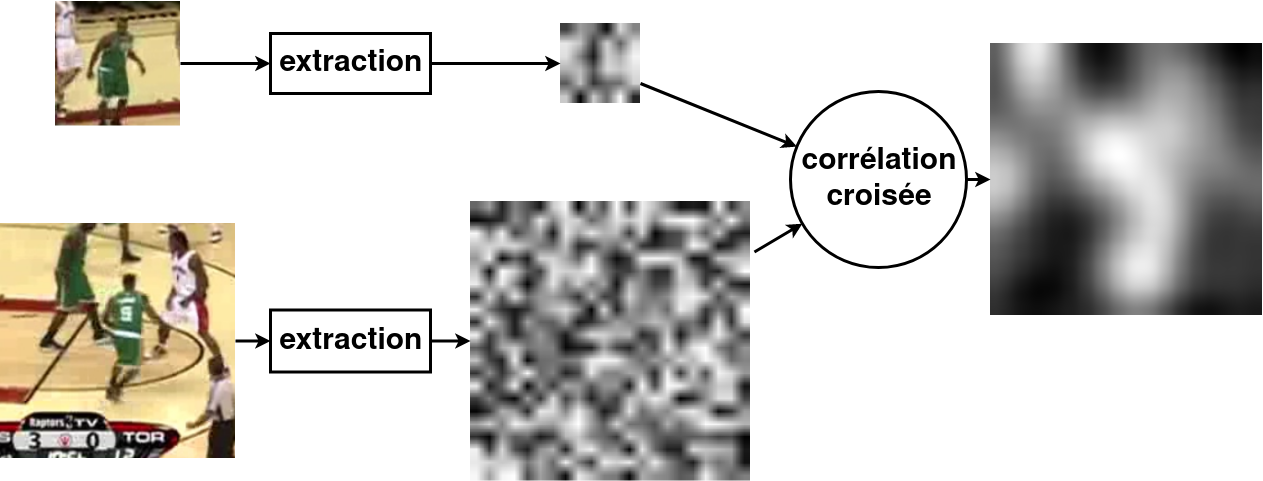
\includegraphics[width=260pt]{images/vids/basket/cross.png}
  \caption{\textbf{Structure spécifique du réseau siamois de l'approche du rapport.} Sur la branche du haut, l'extracteur analyse l'image de initiale de la cible à suivre, en extrait les caractéristiques pour créer le \textit{noyau}. Sur la branche du bas, l'extracteur analyse l'image de recherche. La tête du réseau à droite est une corrélation croisée qui génère les cartes de corrélations. Sur le schéma, la résolution de la carte de corrélation est augmentée.}
  \label{strucutre}
  \end{figure}

On extrait la carte des caractérisitiques de l'image de recherche par le même réseau extracteur que pour le noyau. Une carte de corrélation est ensuite calculée par corrélation croisée entre le noyau du système et la carte de caractérisitiques de recherche. La figure \ref{strucutre} montre la structure générale pour le calcul des cartes de corrélations.

La position du pixel de plus haute intensité sur la carte de corrélation devient l'estimation du centre de la position de l'objet. Seule la position de l'objet est estimée et la taille des \textit{bounding boxes} ne change que par la prise en compte de la taille la zone de recherche. L'algorithme \ref{algo1} résume chacune des grandes étapes de la méthode de suivi. Cette méthode constitue une référence et nous proposons une amélioration dans la partie \textit{\nameref{noyau}}.


\begin{algorithm}
\SetAlgoLined
 $initialiser$ le centre $c$\;
 $\mathcal{K} = extraction($cible$)$\;
 \Pour{image $\mathcal{I}$ dans vidéo}{
  $\mathcal{R} = crop_{\mathcal{I}}(\mathcal{I}, c)$\;
  $\mathcal{F} = extraction(\mathcal{R})$\;
  $\mathcal{C} = correlation(\mathcal{K}, \mathcal{F})$\;
  $c = argmax(\mathcal{C})$\;
 }
\caption{Algorithme de suivi d'objets.\\$\mathcal{K}$ est le noyau. $\mathcal{R}$ est l'image de recherche. $\mathcal{F}$ est la carte de caractérisitiques. $crop_{\mathcal{I}}$ est la fonction qui sélectionne la zone de recherche. La valeur d'interêt est $c$, le centre de l'objet prédit pour chaque étape.}
\label{algo1}
\end{algorithm}




\subsubsection*{Ensembles de données}

La série des bases de données \textbf{VOT} \cite{VOT} font office de références dans le domaine du SOT (\textit{Single Object Tracking}). Il s'agit d'un challenge proposé tous les ans sur un nouveau dataset créé pour l'occasion. Les banques \textbf{OTB-50} et \textbf{OTB-100} \cite{OTB} font aussi office de norme. Cependant, ces banques de données n'ont pas pour vocation à servir à l'entrainement des modèles, mais à la comparaison des performances. Nous utiliserons la banque de données \textbf{GOT-10k} \cite{GOT10K} pour l'entrainement ainsi que pour la validation. Et nous utiliserons OTB-100 pour comparer les performances de nos modèles.

\subsubsection*{Métriques}
\label{metrics}


Il existe différentes métriques pour mesurer les performances des modèles en suivi d'objets qui sont différentes pour les tâches SOT et MOT.

Nous baserons notre étude sur la dualité entre précision et taux de succès pour l'évaluation. Le taux de succès (\textit{succes rate}) consiste à calculer la proportion de temps pendant lequel l'intersection de la prédiction et de la vérité étiquetée dépasse un certain seuil selon l'indice de Jaccard. Un graphique donnera l'évolution du ratio en fonction du seuil, celui-ci variant de 0 à 1. Notons que cette métrique mesure une performance proche de l'espérance du chevauchement moyen (\textit{expected average overlap}), où le chevauchement est l'indice de Jaccard (\textit{Intersection Over Union}). C'est une autre métique classique en VOT.

Cependant cette métrique ne permet pas d'avoir une bonne idée du comportement du suiveur, en effet chaque modèle prédit à la fois une région (\textit{bounding box}) et le centre de l'objet, une métrique basée seulement sur la région proposée de permet pas de mesurer la précision du suiveur. La précision (\textit{precision}) est mesurée par le pourcentage d'images pour lesquelles le centre de l'objet prédit et le vrai centre sont espacés d'une distance inférieure à un seuil donné. Là encore, un graphique donnera la précision en fonction de ce seuil.

Comme un graphique ne peut pas donner une méthode directe de comparaison des suiveurs, nous utiliserons l'aire sous la courbe (\textit{AUC}) de précision pour classer les modèles. 

\subsubsection*{Méthode d'apprentissage de l'extracteur}

Pour l'apprentissage, nous construisons des paires aléatoires d'images du même objet séparées par un nombre aléatoire de \textit{frames} dans la vidéo. Pour des raisons de cohérence de l'apparence des couples d'entrainement, les images ne peuvent pas être séparées de plus de 100 \textit{frames}. De chaque couple, on extrait les cartes de caractérisitiques fournies par le modèle extracteur apprenant. La tête calcule la corrélation croisée de ces cartes. La carte de corrélation obtenue est alors comparée aux données étiquettée : les coordonnées réelles de l'objet cible dans l'image de recherche.

On ne peut pas directement constuire une fonction de coût basée sur la comparaison de la carte corrélation (données matricielles) et les coordonnées de la cible étiquettées vectorielles (\textit{bounding boxes}) puisqu'elle ne sont pas de même nature : on doit transformer le problème en un problème de classification.

\begin{figure}[!h]
\centering

\includegraphics[width=50pt]{images/loss/predict.png}
\hspace{0.7cm}

\includegraphics[width=50pt]{images/loss/target.png}
\caption{\textbf{Visualisation des entrées de la fonction de coût.} À gauche, une carte de corrélation prédite. À droite, l'objectif auquel la comparer.}
\label{loss_corr}
\end{figure}

Pour cela on construit à partir de coordonnées étiquettées une carte de même dimension que la carte des corrélations telle qu'on associe aux pixels proches da la position de la cible (\textit{connue}) une valeur $y_{p}=1$, et aux pixels éloignés une valeur $y_{p}=0$. La distance entre la position de la cible et les pixels négatifs est un hyper-paramètre du suiveur $r_{neg}$. Un exemple de carte ainsi construite est montré figure \ref{loss_corr}. Le problème revient à un problème de classification classique sur chacun des pixels. On utilise comme fonction de coût $L$ une entropie croisée binaire sur chaque pixel de chaque image d'un batch :

$$l_p = y_{p} \cdot \log \sigma\left(x_{p}\right)+\left(1-y_{p}\right) \cdot \log \left(1-\sigma\left(x_{p}\right)\right)$$

$$L = \sum_{\mathcal{I} \in batch} \sum_{p \in \mathcal{I}} l_p$$

Cependant, chaque carte de labels a un nombre très inégal d'instances positives et négatives puisque seule une petite zone de chaque image correspond effectivement à la présence d'un objet. Un tel comportement peut avoir des effets néfastes déstabilisateurs sur l'apprentissage \footnote{Le modèle aurait tendance à prédire qu'aucun des pixels ne correspond à la cible. Comme les pixels tels que $y_{p}=0$ sont très majoritaires, la fonction de coût admettrait un minimum local pour la prédiction \textit{facile} $\forall p \hspace{0.5em} x_{p}=0$, ce qui rendrait la convergence plus difficile.}. Pour prendre cela en considération, on utilise un coût équilibré (\textit{Class-Balanced Loss}) :

$$L = \sum_{\mathcal{I} \in batch} \sum_{p \in \mathcal{I}} w_{p}l_p$$

où $$w_{p} = \frac{1}{\sum_{\mathcal{I} \in batch}p_{\{+/-\}}} $$

%\frac{\nu_{p}}{\norm{\nu_{p}}} \text{ et } \nu_{p}

où $p_{\{+/-\}}$ est égal au nombre d'instances positives \textit{(resp. négatives)} dans l'image si $y_{n}$ est postive \textit{(resp. négative)}. \\

À l'exception des modifications de valeurs dans le cardre des expérimentations (qui seront mentionnées), on utilise les hyper-paramètres d'apprentissage proposés dans le papier originel du siamFC \cite{siamfc}. Il s'agit en particulier : d'une taille de \textbf{mini-batch de 8 couples} de cartes de corrélations, une \textbf{régulation $L_2$ de 5e-4}, un \textbf{SGD de moment 0.9} et de \textbf{taux d'apprentissage exponentiellement décroissant de 1e-3 à 1e-5}. Les calculs sont effectués sur GPU GeForce RTX3070, pour des temps de calcul de l'ordre de 10h pour 100 passes. Le nombre de passes effectif est déterminé par \textit{early stopping} et dépend des expérimentations.


\subsubsection*{Architecture}

L'architecture que nous utilisons en tant que référence est celle proposée par L.Bertinetto \cite{siamfc}. Dans cette architecture, chaque réseau extracteur de caractéristiques est construit sur la base des extracteurs AlexNet \cite{alexnet}, auquel on ajoute des couches de \textit{Batch Normalization}. L'architecture de l'extracteur est proposée sur la figure \ref{archi_ref}. La tête de l'architecture est une corrélation croisée, et elle n'admet aucun paramètre apprenable.

Un des buts de ce travail est d'étudier la pertinence de cette architecture de référence. On se concentre en particulier sur l'utilisation des \textit{Batch Normalization} et du nombre optimal de couches dans le réseau. Pour l'étude des \textit{Batch Normalization} notre approche expérimentale sera de comparer l'apprentissage puis les performances de la structure totale avec et sans les \textit{Batch Normalization}, tout en conservant l'architecture de référence en ce qui concerne les autres composants du réseau. Pour l'étude du nombre optimal de couches, on teste des architectures en ajoutant successivement des couches. Les différentes architectures testées sont présentées en annexe \ref{annexe_archis}.

\begin{figure*}[!h]
  \centering
  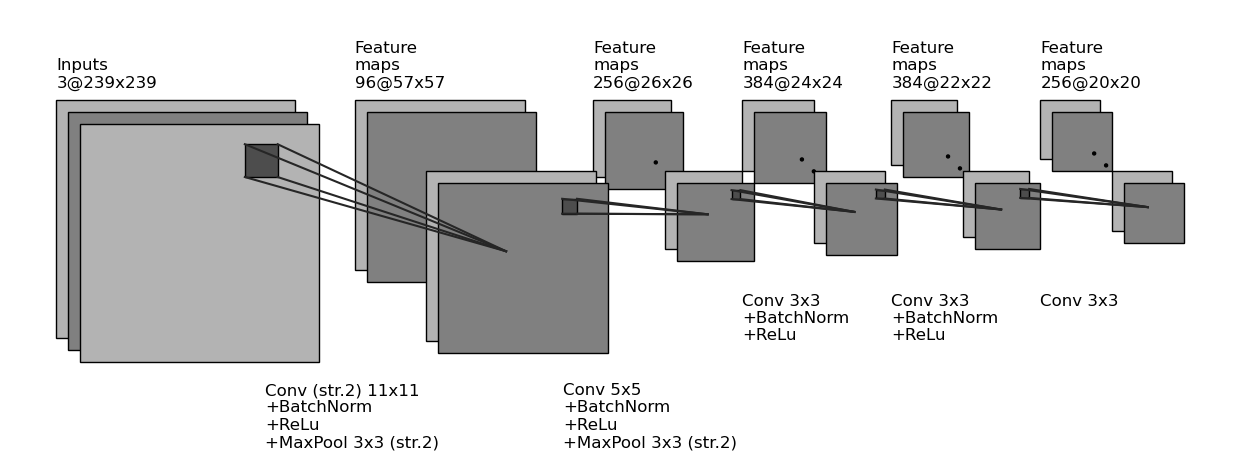
\includegraphics[height=160pt]{images/archis/convnet_cnn5.png}
  \caption{\textbf{Structure de référence de l'extracteur de caractéristiques qui est utilisé dans chacune des branches du modèle siamois.} La tête du réseau qui effectue la corrélation n'est pas représentée sur le schéma.}
  \label{archi_ref}
  \end{figure*}


Chacune des expérimentations se fait en optimisant les autres hyper-paramètres par recherche manuelle (la régulation $L_2$, le moment, et le taux d'apprentissage) sur l'ensemble de validation. Chaque expérience est ré-itérée cinq fois, et les performances à comparer sont mesurées sur l'ensemble de test puisqu'il ne s'agit pas d'un réglage d'hyper-paramètre, et que l'on souhaite prendre en compte la meilleure estimation possible de l'erreur de généralisation.


\subsubsection*{Amélioration du noyau}
\label{noyau}

La méthode de référence compare, à chaque instant, l'image de l'objet que l'on cherche à l'image dans laquelle on cherche l'objet. Or, cette méthode n'est pas optimale dans plusieurs cas, notamment lorsque que l'objet change de apparence ou lorsque plusieurs objets sont proches et se ressemblent beaucoup. Ces situations seront discutées dans la partie \textit{\nameref{echecs}}. Dans ce rapport, on propose d'étudier une amélioration qui consiste à ne pas seulement chercher l'image de la cible telle qu'elle a été donnée lors de l'initialisation de la séquence, mais de chercher aussi la cible telle qu'elle a été détectée durant la séquence.

Pour cela, on introduit un deuxième noyau, que l'on appelera \textit{noyau glissant} (noté $\mathcal{K}_{glissant}$). Il s'agit d'un historique des apparences de l'objet détecté dans les dernière images de la vidéo. La mise à jour de ce noyau est régie par un nouvel hyper-paramètre $\gamma$, le noyau sera équivalent à une moyenne mobile exponentielle des dernières cartes de caractéristiques associées à la cible. La mise à jour sera de la forme : 
$$\mathcal{K}_{glissant} += \gamma(\mathcal{K}_{\mathcal{I}}-\mathcal{K}_{glissant})$$
où $\mathcal{K}_{\mathcal{I}}$ est la carte de caractéristiques calculée à partir de la dernière détection de l'objet.\\

Comme dans la méthode de référence, la position de l'objet est estimée par l'argument maximal des cartes de corrélations du noyaux et de l'image de recherche. Dans cette nouvelle méthode, il y a deux noyaux, donc deux cartes de corrélation, et donc deux vecteurs de coordonnées pour l'estimation de la position de l'objet (notés $c_{ref}$ et $c_{glissant}$). L'estimation retenue pour le suivi sera une moyenne $c$ pondérée par $\beta$ des deux vecteurs :
$$c = \beta c_{ref} + (1-\beta) c_{glissant}$$

Cette nouvelle méthode est résumée par l'algorithme \ref{algo2}. Dans la partie expérimentale, nous comparerons les résultats obtenus par la méthode de référence et la méthode modifiée. De la même manière que dans le paragraphe précédent, chacune des expérimentations se fait en optimisant les autres hyper-paramètres (la régulation $L_2$, le moment, le taux d'apprentissage, et maintenant $\beta$ ainsi que $\gamma$) par recherche manuelle sur l'ensemble de validation.

\begin{algorithm}
\label{algo2}
\textbf{Soient} $\gamma$ et $\beta$ hyper-paramètres.

\SetAlgoLined
 $initialiser$ le centre $c$ \;
 $\mathcal{K} = extraction($cible$)$\;
 $\mathcal{K}_{glissant} = \mathcal{K}$\;
 \Pour{image $\mathcal{I}$ dans vidéo}{
  $\mathcal{R} = crop_{\mathcal{I}}(\mathcal{I}, c)$\;
  
  $\mathcal{F} = extraction(\mathcal{R})$\;
  
  $\mathcal{K}_{\mathcal{I}} = crop_{\mathcal{K}}(\mathcal{F})$\;
  
  $\mathcal{C}_{ref} = correlation(\mathcal{K}, \mathcal{F})$\;
  $\mathcal{C}_{glissant} = correlation(\mathcal{K}_{glissant}, \mathcal{F})$\;
 
  
  $c_{ref} = argmax(\mathcal{C}_{ref})$\;
  $c_{glissant} = argmax(\mathcal{C}_{glissant})$\;
  
  $c = \beta c_{ref} + (1-\beta) c_{glissant}$\;
  
  $\mathcal{K}_{glissant} += \gamma(\mathcal{K}_{\mathcal{I}}-\mathcal{K}_{glissant}$)\;
  
 }
\caption{Amélioration de l'algorithme \ref{algo1}, avec les mêmes notations. La fonction $crop_{\mathcal{K}}$ effectue la même action que $crop_{\mathcal{I}}$ mais sur le noyau au lieu des images.}
\end{algorithm}




\section*{Expérimentations}

\subsubsection*{Résultats de référence}

Notre implémentation de l'approche de référence (architecture du siamFC \cite{siamfc} et algorithme \ref{algo1}) fournit des résultats qui correspondent à l'état de l'art de 2016, date de publication du siamFC. Compte tenu des métriques expliquées dans la partie \textit{\nameref{metrics}}, les courbes de précision et de taux de succès sont disponibles sur la figure \ref{courbes_BN}, il s'agit des courbes notées \textit{avec BN}. L'aire sous la courbe de précision (\textit{AUC}) est de \textbf{0.741}, et le score de succès pour un seuil de 20 est de \textbf{0.553}. Des exemples d'instances de suivis sur les séquences de test sont donnés en annexe \ref{annexe_exemples}. Ces résultats cohérents donnent une bonne référence à laquelle comparer les études sur les architectures et sur le noyau glissant. Pour bien comprendre le comportement du suiveur, la partie suivante propose une étude des cas d'échecs typiques du suiveur.

\subsubsection*{Étude des cas d'échecs}
\label{echecs}

Une étude des séquences donnant les moins bons résultats met en avant quatre cas d'échec classiques : \textit{\nameref{proches}}, \textit{\nameref{obstructions}}, \textit{\nameref{aspect}}, et \textit{\nameref{falsh}}.


\subsubsection*{a. Objets similaires proches}
\label{proches}

De nombreux échec sont dûs à une confusion du suiveur entre deux objets très similaires dans la vidéo. Ceci s'explique par le fait que le suiveur ne se base que sur la similaraité de l'objet suivi avec l'image de la cible fournie au début de la vidéo. La cohérence du suivi n'est assuré que par la proximité de l'objet d'une image à la suivante imposée par la petite taille de l'image de recherche centrée autour de la dernière position de l'objet. Or si par défaillance le suiveur change de cible, alors il ne pourra pas retrouver la cible orginale qui sera trop loin. Cela mène aussi à des situations où le suiveur se bloque sur des objets en arrière-plan sans pouvoir rattrapper la vraie cible.


\subsubsection*{b. Obstructions longues}
\label{obstructions}

\begin{figure}[!h]
  \centering
  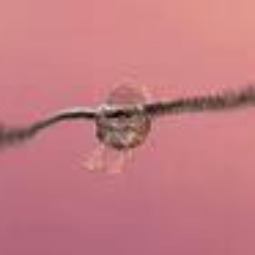
\includegraphics[width=50pt]{images/vids/bird/search/000117.png}
  
\includegraphics[width=50pt]{images/vids/bird/search/000162.png}
  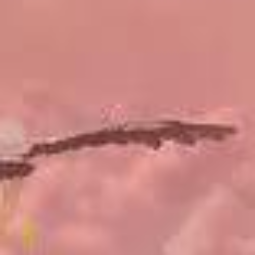
\includegraphics[width=50pt]{images/vids/bird/search/000186.png}\\
  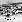
\includegraphics[width=50pt]{images/vids/bird/pre-corr/000117.png}
  
\includegraphics[width=50pt]{images/vids/bird/pre-corr/000162.png}
  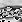
\includegraphics[width=50pt]{images/vids/bird/pre-corr/000186.png} 
  \caption{\textbf{Exemple d'obstruction longue (dataset de test OTB).} En haut, les images de recherche dans lesquelles on doit trouver la cible, ici l'oiseau. Elles sont ordonnées temporellement mais non consécutives. En bas, les cartes de corrélations associées. On observe que pendant l'obstruction la carte de corrélation n'est pas porteuse d'information : la valeur de la corrélation est constante sur toute l'image. Le suiveur aura tendance à rester dans le même position, c'est-à-dire à toujours prédire l'objet au centre de l'image de recherche.}
  \label{obstruct}
  \end{figure}

Comme pour beaucoup de méthodes de suivi, la robustesse aux obstructions longues est un problème majeur. C'est un problème beaucoup plus complexe dans le cas des tâches MOT \textit{Mutli Object Tracking} que pour les tâches SOT \textit{Single Object Tracking}. Pour le siamFC, en cas d'obstructions longues et en l'absence d'information sémantique sur les cartes de caractéristiques celles-ci auront tendance à être naturellement constantes sur toute l'image. Les cartes de corrélations ne seront donc pas porteuses d'informations, et par défaut, la zone de détection restera là où elle était avant l'obstruction. Une telle situations est montrée sur la figure \ref{obstruct}. Le ré-accrochage de la cible dépend donc du mouvement de l'objet dans la vidéos \textit{pendant l'obstruction}. Si l'objet reste dans une zone proche de la zone dans laquelle le suiveur l'a perdu, ce dernier pourra retrouver la cible à suivre. Notons que l'objet doit rester fixe dans le repère de l'image, ce qui signifie que tout mouvement de la caméra pendant l'obstruction pourra faire perdre de vue l'objet au suiveur. 






\subsubsection*{c. Changements d'aspect de la cible}
\label{aspect}

Un cas fréquent d'échec survient quand l'objet change d'apparence. En particulier, dans la plupart des vidéos \textit{naturelles}, les objets ne sont pas vus du même angle pendant toute la vidéo. Or, avec la méthode de référence, l'objet que l'on cherche doit être similaire sémantiquement à l'objet l'objet tel qu'il est donné à l'initialisation de la séquence. Malgrè le haut niveau d'abstraction auquel s'effectue la comparaison, le modèle peine à reconnaitre certains objets (comme une personne de dos). Un exemple extrême provenant de la base de données de validation est disponible sur la figure \ref{coupons}. 
Ce problème de changement d'aspect de la cible est l'une des raisons pour lesquelles nous avons proposé la mémorisation des noyaux, qui permet de garder en mémoire les toutes dernières apparences de l'objet.

\begin{figure}[!h]
  \centering
  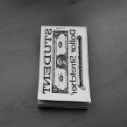
\includegraphics[width=50pt]{images/vids/coupon/kernel/000001.png}
  \vspace{5pt}\par
  \hrule
  \vspace{5pt}\par
  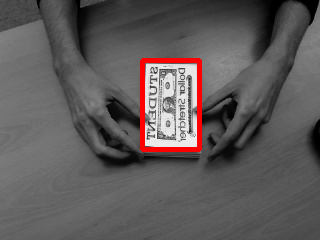
\includegraphics[width=70pt]{images/vids/coupon/000039.png}
  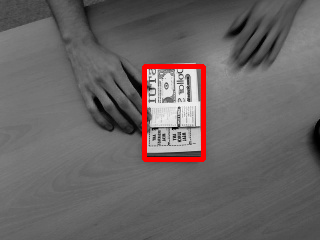
\includegraphics[width=70pt]{images/vids/coupon/000070.png}
  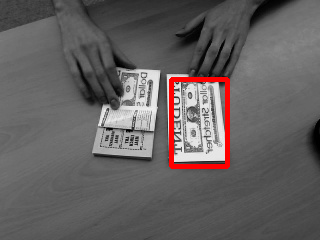
\includegraphics[width=70pt]{images/vids/coupon/000159.png} 
  \caption{\textbf{Exemple d'une séquence qui comporte un changement d'aspect.} En haut, l'image initiale de la cible à suivre. En bas, des images de la séquences ordonnée temporellement et non consécutives. Dans la vidéo, un manipulteur plie le billet en deux, l'objectif du suiveur est de suivre le billet après son pliage. Après le pliage, le billet à suivre ressemble moins au noyau que les autres billets, c'est donc une séquence très difficile pour un suiveur, en particulier quand celui-ci n'a pas d'historique des apparences de la cible.}
  \label{coupons}
  \end{figure}

\subsubsection*{d. Flash}
\label{falsh}

\begin{figure}[!h]
  \centering
  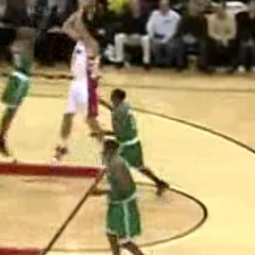
\includegraphics[width=60pt]{images/vids/basketflash/650/000649.png}
  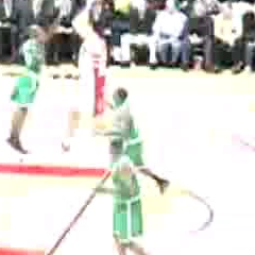
\includegraphics[width=60pt]{images/vids/basketflash/650/000650.png}
  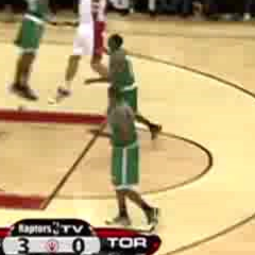
\includegraphics[width=60pt]{images/vids/basketflash/650/000651.png}\\
  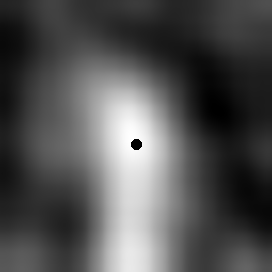
\includegraphics[width=60pt]{images/vids/basketflash/650/corr/000649.png}
  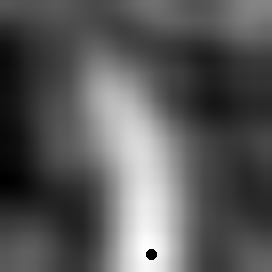
\includegraphics[width=60pt]{images/vids/basketflash/650/corr/000650.png}
  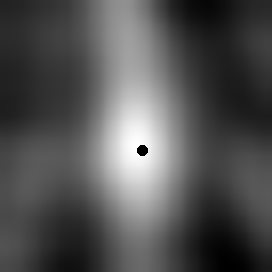
\includegraphics[width=60pt]{images/vids/basketflash/650/corr/000651.png} 
 
 \hfill
 
  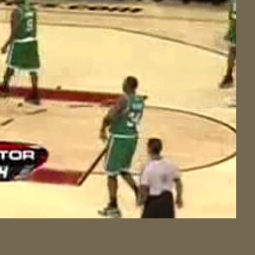
\includegraphics[width=60pt]{images/vids/basketflash/700/000699.png}
  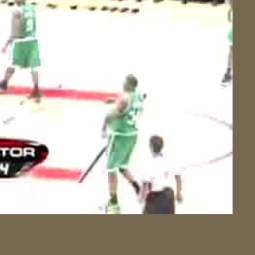
\includegraphics[width=60pt]{images/vids/basketflash/700/000700.png}
  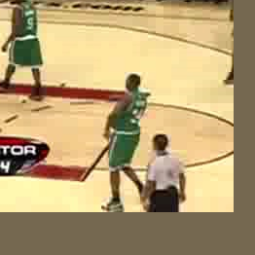
\includegraphics[width=60pt]{images/vids/basketflash/700/000701.png}\\
  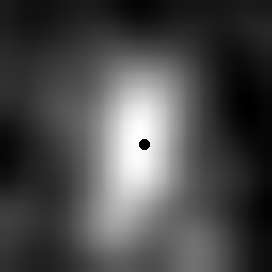
\includegraphics[width=60pt]{images/vids/basketflash/700/corr/000699.png}
  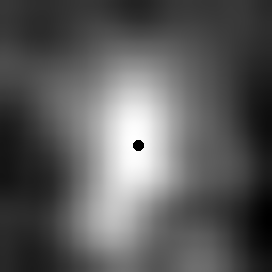
\includegraphics[width=60pt]{images/vids/basketflash/700/corr/000700.png}
  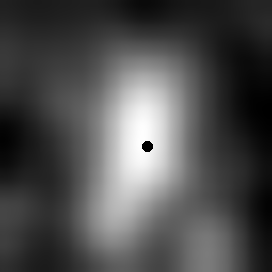
\includegraphics[width=60pt]{images/vids/basketflash/700/corr/000701.png} 
  \caption{\textbf{Effet d'un flash sur les cartes de corrélations.} En haut et en bas, il s'agit de deux séquences dont les images sont consécutives. En bas, leurs cartes de corrélations associées dont le point noir indique le maximum. Dans les deux cas, le flash modifie de manière non uniforme les cartes de corrélations (elles sont \textit{blanchies}). Dans la séquence du haut, le flash fait perdre la cible au suiveur, mais l'image du bas montre que ce n'est pas toujours le cas. }
  \label{flash}
  \end{figure}


Certaines vidéos comportent des flash (d'appareil photo pour la plupart). Un bon suiveur doit pouvoir être robuste aux flash car c'est une situation courante. La figure \ref{flash} montre l'effet d'un flash sur l'une des images de la vidéo. Dans l'espace des images, un flash va blanchir toute l'image, rendant difficile à distinguer les objets. Dans l'espace des cartes de corrélations, on observe que les flash ont tendance augmenter la valeur de corrélation un peu partout sur la carte, mais de manière non uniforme. Ceci provoque des  irrégularités dans les cartes de corrélation, et donc des changements de cibles du suiveur dans les cas de malchance.


\subsubsection*{Architecture}

\subsubsection*{a. Effet des normalisations par batch}

Les résultats de l'expérimentation conduisant à étudier l'impact des normalisation par batch montrent que celles ci permettent d'augmenter significative la qualité du suiveur, autant en précision qu'en taux de succès. Les résultats sont donnés sur la figure \ref{courbes_BN}.


\begin{figure}[h!]
\centering
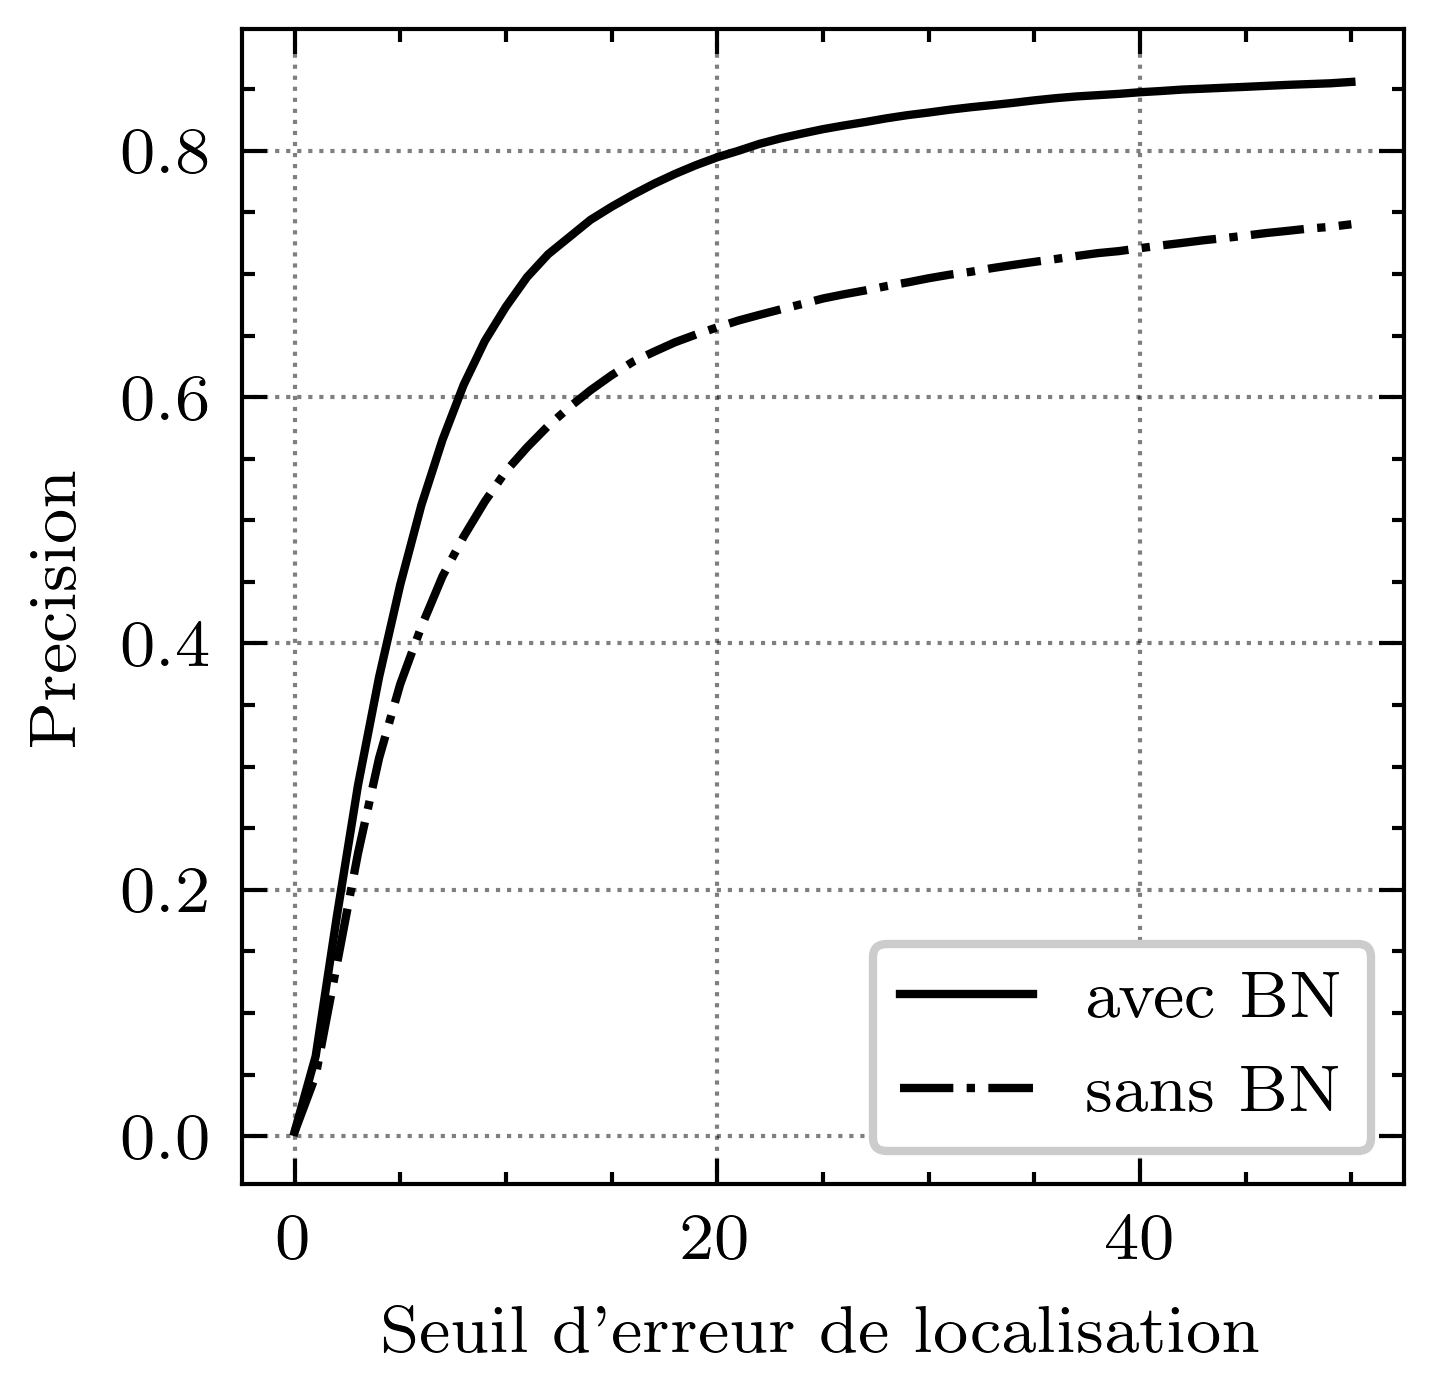
\includegraphics[width=125pt]{images/BN/courbes_pre.png} 
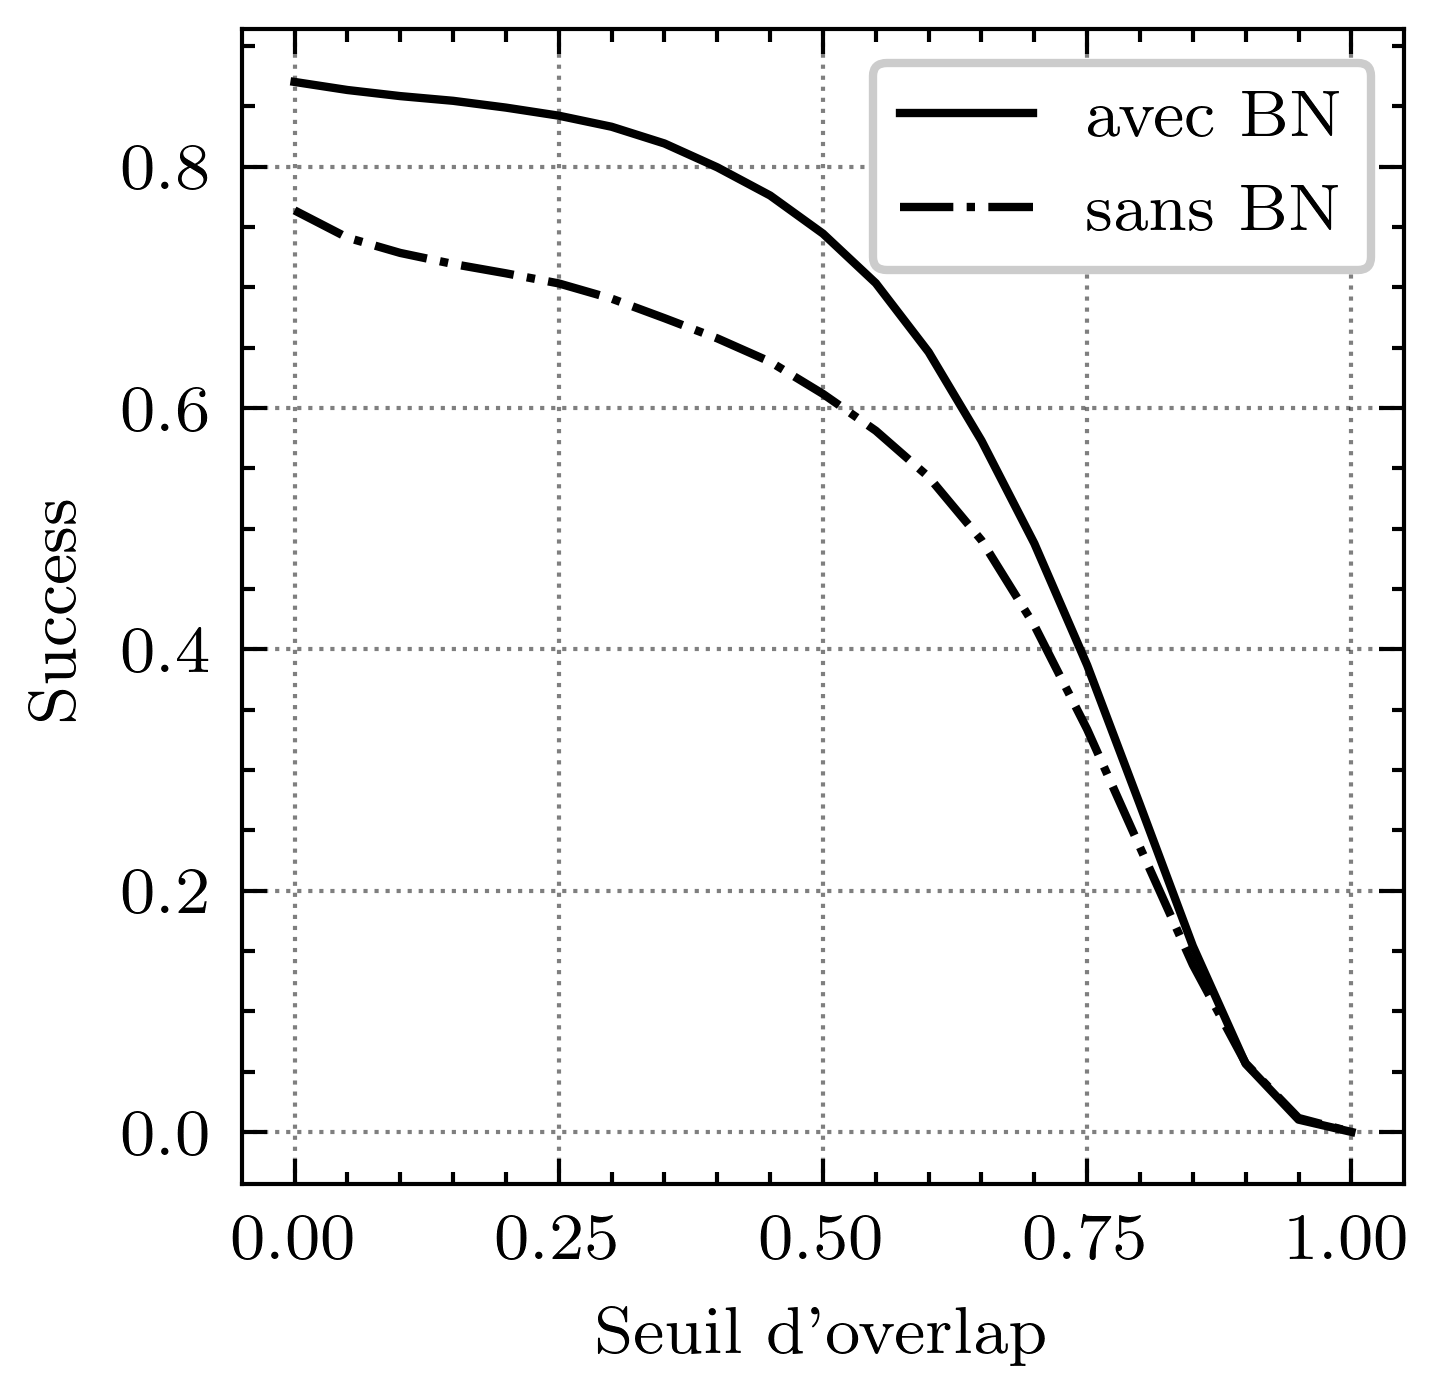
\includegraphics[width=125pt]{images/BN/courbes_succ.png} 
\caption{\textbf{Effet des normalisations par batch sur les performances.} Performance du suiveur équipé d'un extracteur à 5 couches de type AlexNet (modèle de référence) avec et sans normalisations par batch (BN).}
\label{courbes_BN}
\end{figure}




\begin{figure}[!h]
  \centering
  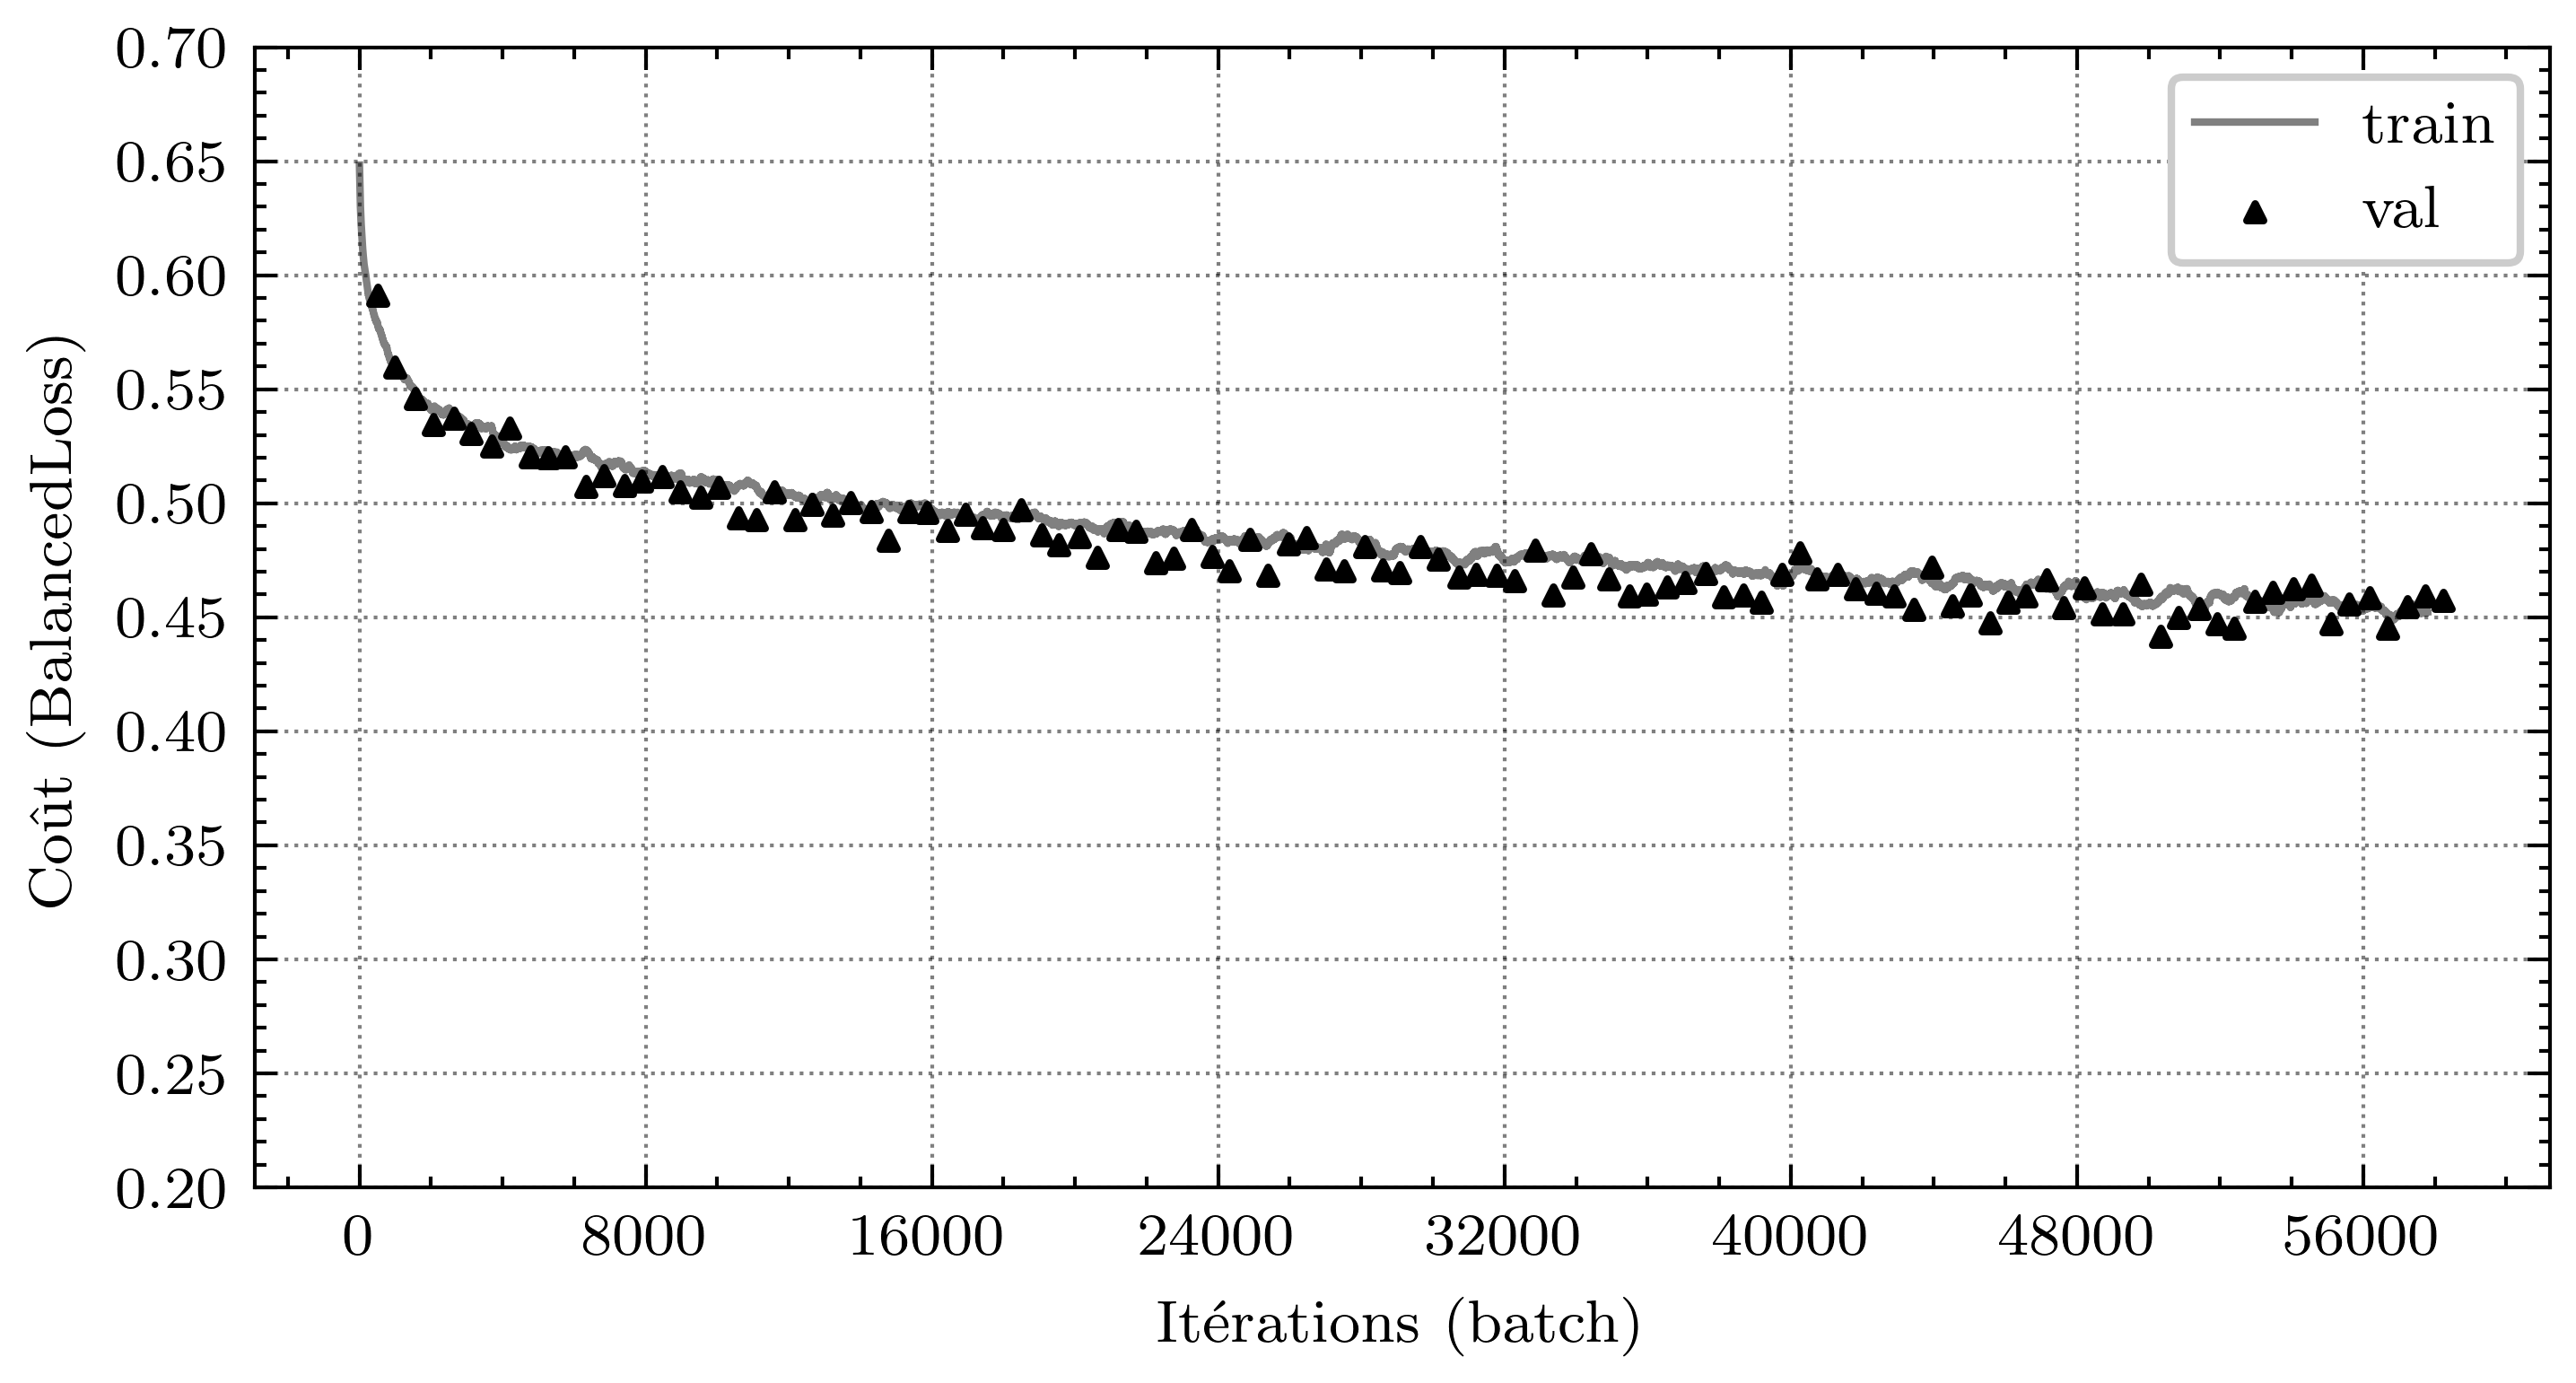
\includegraphics[width=260pt]{images/BN/courbes_sansBN.png} 
  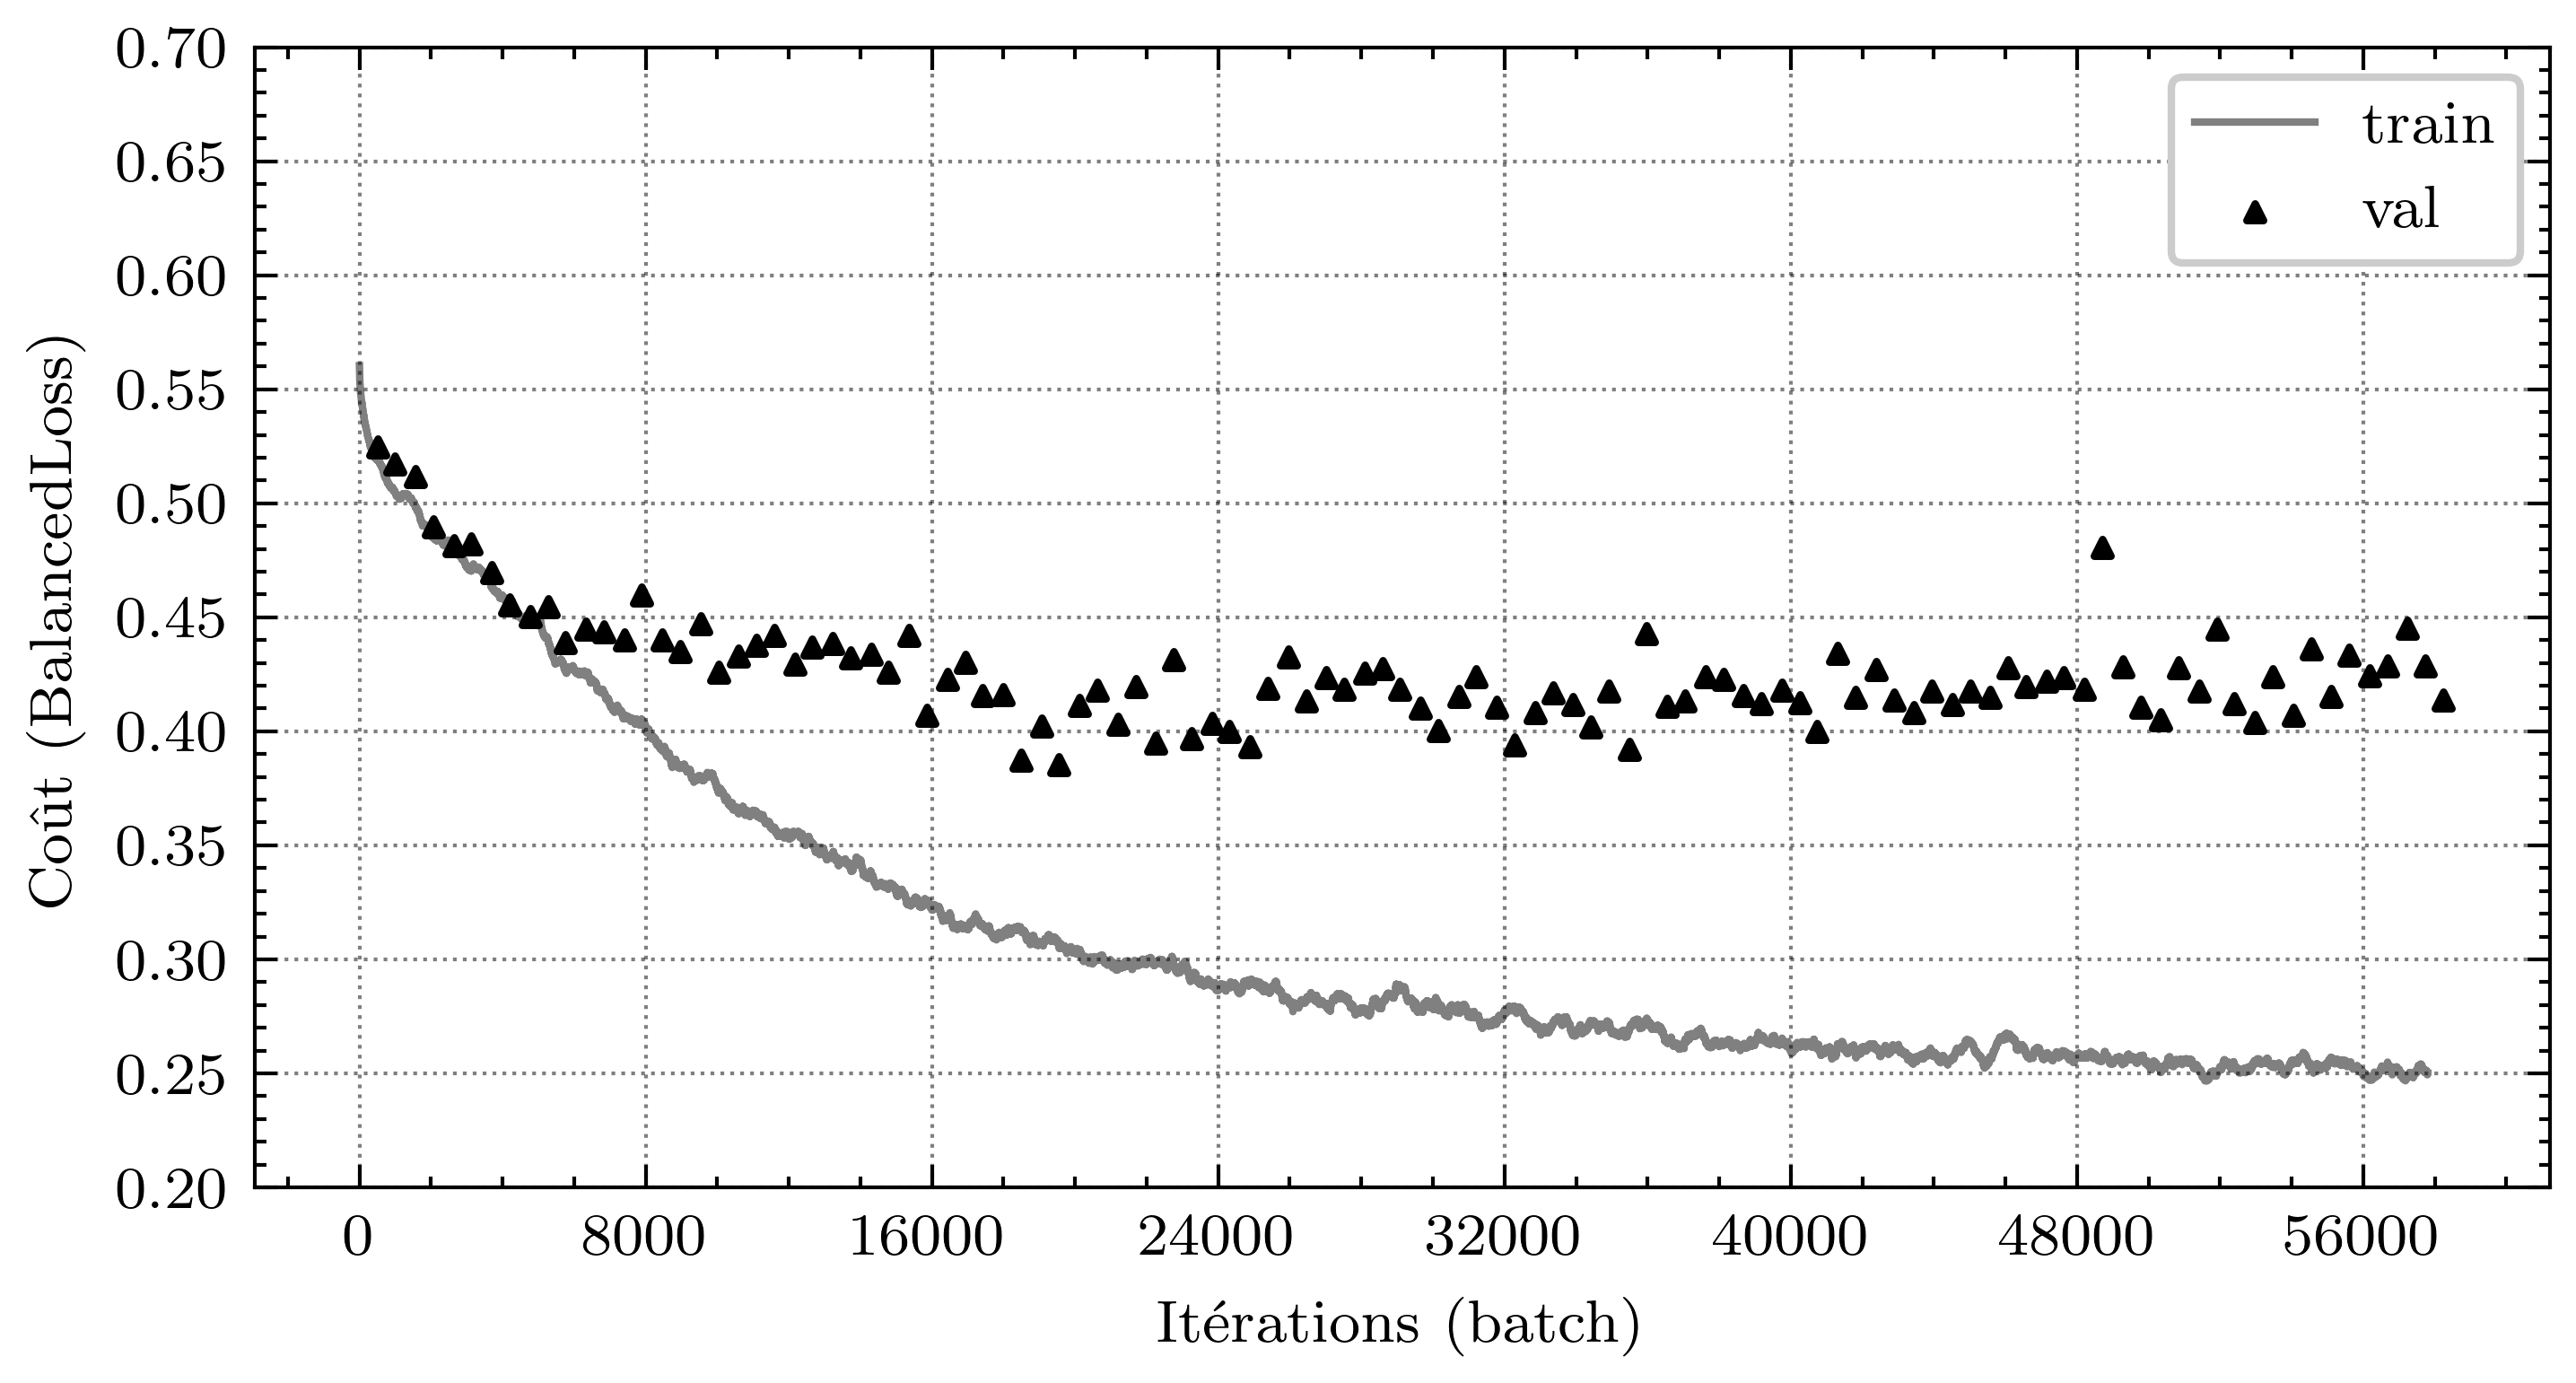
\includegraphics[width=260pt]{images/BN/courbes_avecBN.png} 
  \caption{\textbf{Comparaison du comportement des modèles au cours de l'apprentissage en fonction de la présence des normalisations par batch.} L'étiquette \textit{train} correspond au coût en entrainement, et \textit{val} est le coût en validation. En haut, l'apprentissage sans normalisation par batch. En bas, l'apprentissage avec les normalisations. L'entrainement est accéléré par les normalisations et la performance de généralisation est améliorée.}
  \label{courbes_BN_train}
  \end{figure}
  
On peut aussi noter qu'en plus d'améliorer la performance sur les données de test, les normalisations par batch accélèrent fortement la convergence lors de l'apprentissage comme on le voit sur la figure \ref{courbes_BN_train} qui montre l'évolution de l'apprentissage sur les premières itérations. Cela s'explique par la réduction de \textit{covariance shift} décrite par S.Ioffe et al. \cite{ioffe2015batch} même si le sujet est encore discuté \cite{santurkar2019does}. La suppression des \textit{Batch Normalization} diminue légèrement le temps d'inférence du modèle, cependant cela ne suffit pas à justifier une telle perte de performance. Finalement, l'architecture ne peut pas être améliorée en supprimant les normalisations par batch.


\subsubsection*{b. Nombre de couches}

Les résultats de l'expérimentation conduisant à étudier l'impact du nombre de couches comme définie à la section précédente montrent que la performance en fonction du nombre de couche passe par un maximum pour 4 couches. Les trois indicateurs retenus (taux de succès, score de succès, et précision), admettent leur maximum pour la même configuration. Ces résultats sont présentés sur la figure \ref{courbes_fctlay_prec}. Il semble qu'il soit légèrement plus efficace d'utiliser le réseau à 4 couches que l'on a défini plutôt que le réseau à 5 couches qui constituait le modèle de référence. Il serait intéressant de pousser l'étude en vérifiant si cet effet se produit sur d'autres banques de vidéos, et en mettant en relation cet effet avec la \textit{difficulté} des séquences.

\begin{figure}[!h]
  \centering
  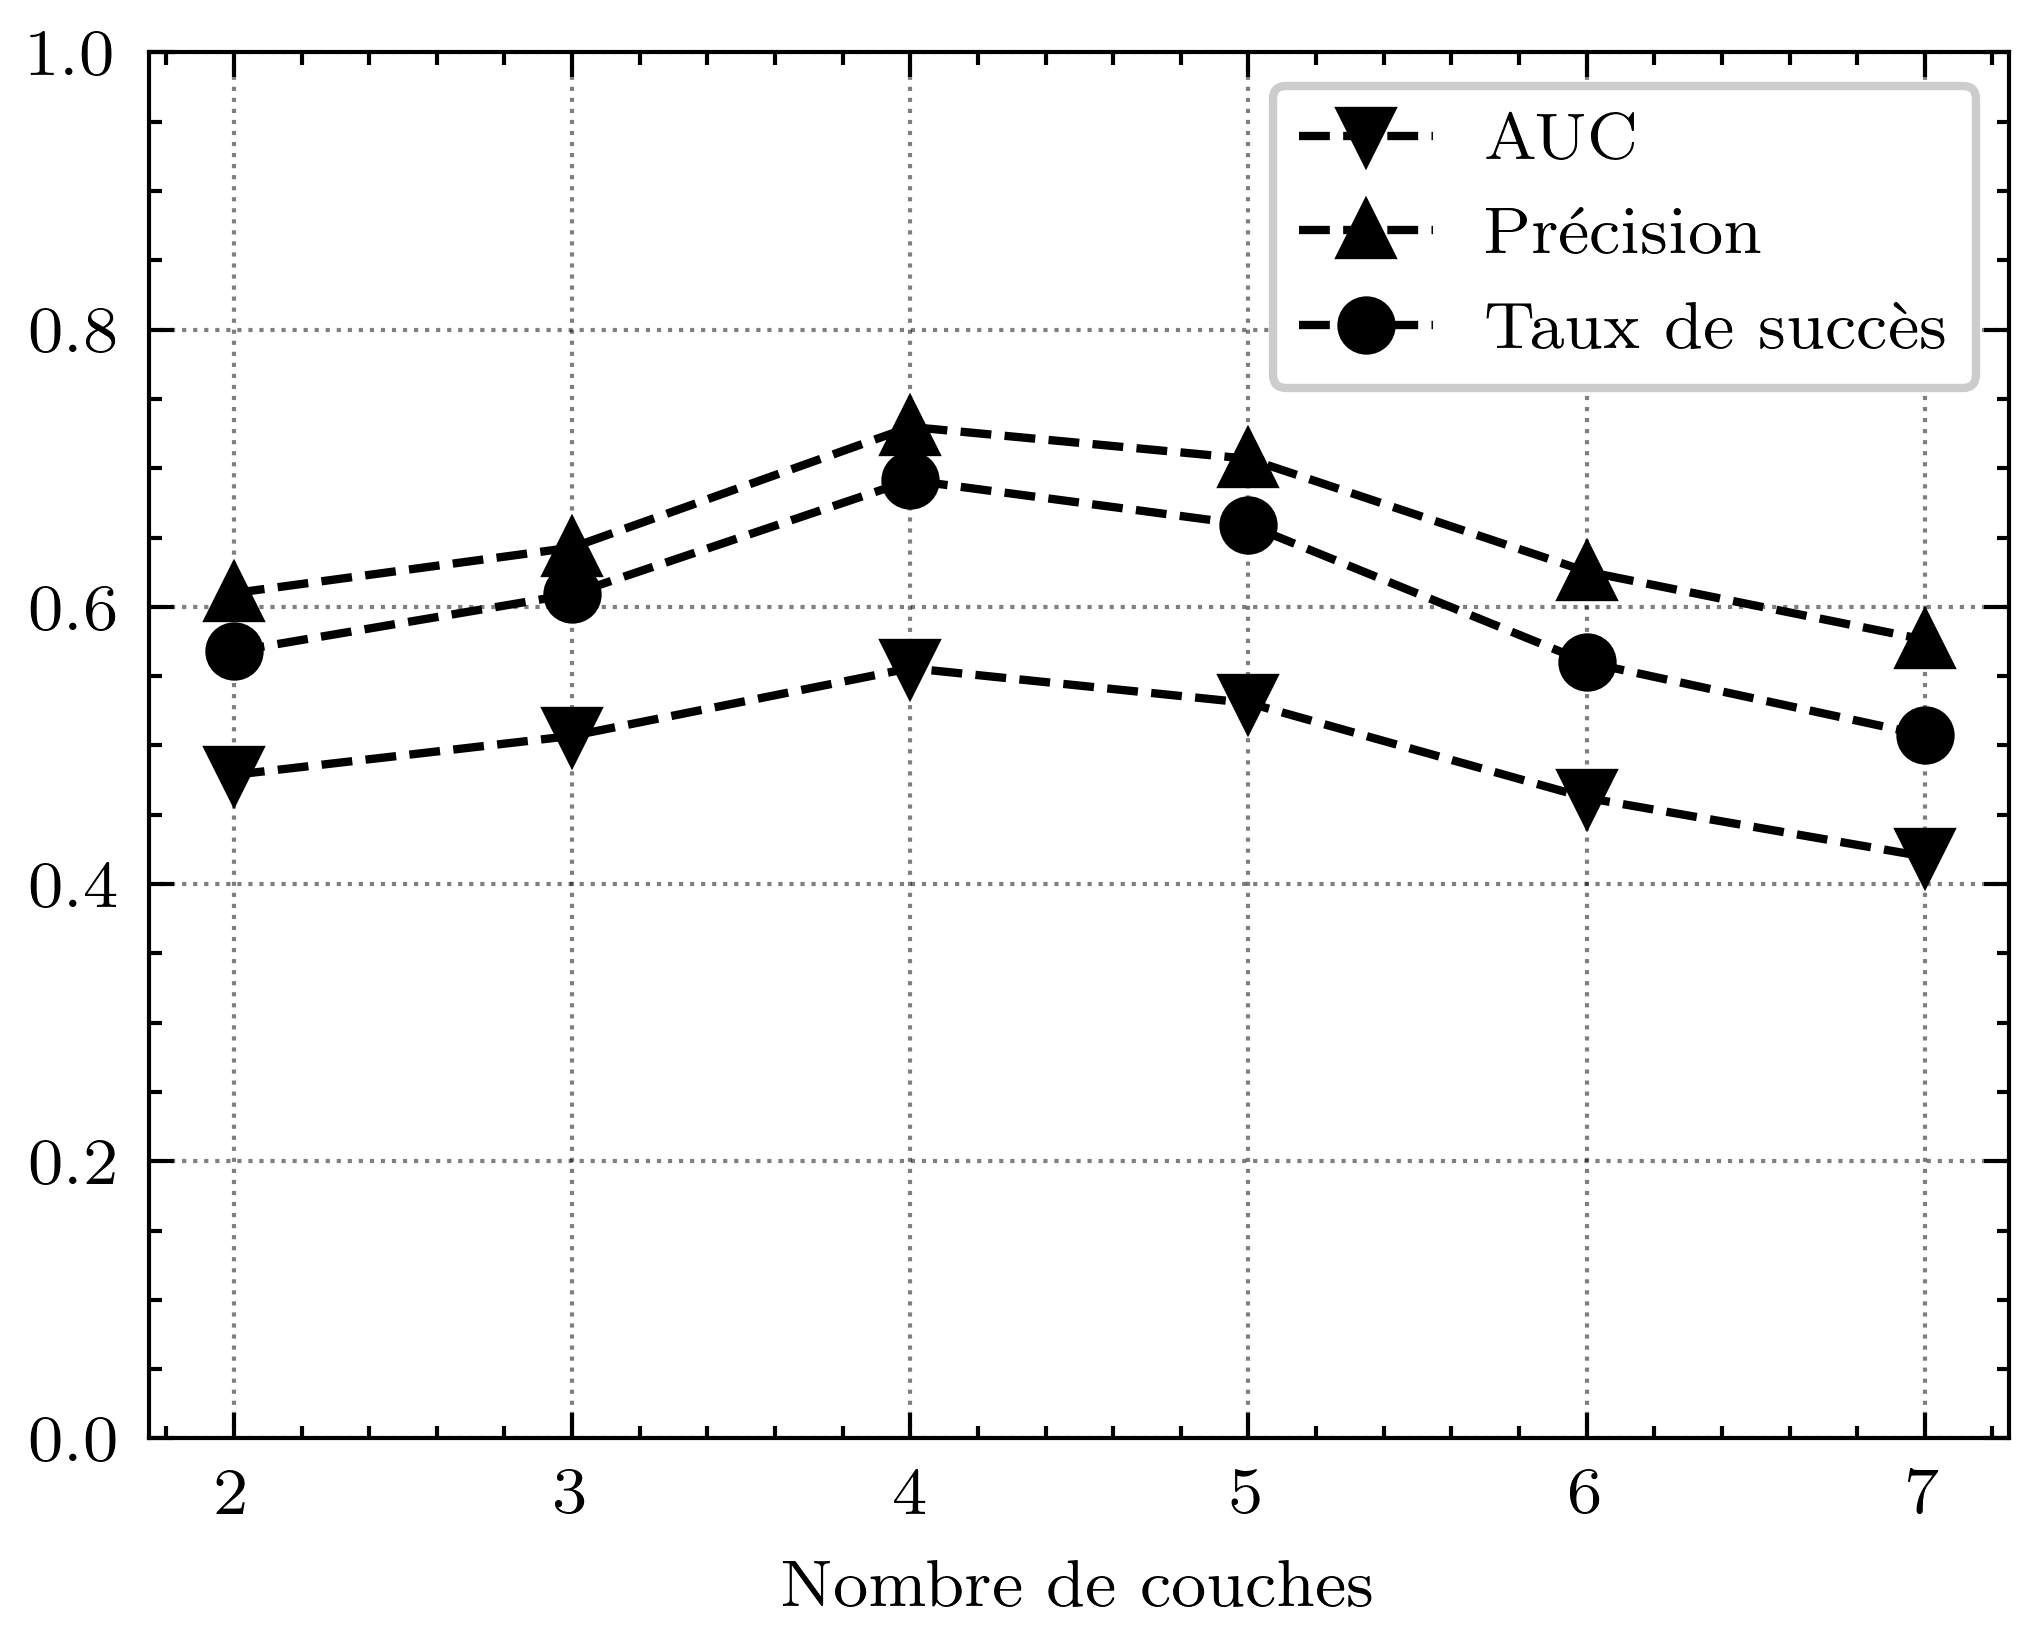
\includegraphics[width=200pt]{images/layers/courbes_fctlay_perfs.png} 
  \caption{\textbf{Performances du suiveur en fonction du nombre de couches de l'extracteur.} Les significations des métriques sont données dans la partie \textit{\nameref{metrics}}. En particulier, \textit{Précision} est la précision pour un seuil de 20, \textit{AUC} est l'aire sous la courbe de succès, et le \textit{Taux de succès} est défini pour un seuil de 0.5. Les détails des architectures utilisées sont données en annexe \ref{annexe_archis}. On observe des performances maximales pour l'architecture à 4 couches, puis 5 couches.}
  \label{courbes_fctlay_prec}
  \end{figure}

Les mauvaises performances des modèles qui comportent peu de couches s'expliquent par une complexité trop faible, qui implique une difficulté à modéliser correctement la tâche. En effet la comparaison des images se fait à un niveau sémantique, il est donc nécessaire de laisser le réseau monter en niveau d'abstraction avant de comparer les cartes de caractérisitiques.

De la même manière, les performances du modèle se déteriore si on lui ajoute trop de couches. Cela s'explique par un sur-apprentissage sur les données d'entrainement. De plus l'ajout de couches augmente beaucoup le temps d'inférence du modèle. Notons enfin que nous avons expérimenté l'utilisation d'un extracteur de ResNet51 \cite{he2015deep} (modèle entier sans la tête de classification), ce qui a conduit, sans surprise, à un fort sur-apprentissage et des performances drastiquement diminuées en validation. 




\subsubsection*{Amélioration du noyau}

\subsubsection*{a. Analyse quantitative}

Les résultats de l'amélioration du noyau grâce au noyau glissant montrent que les performances sont un peu améliorées par ce nouveau noyau. Comme le montre la figure \ref{courbes_prec2}, ces améliorations sont cependant à relativiser. Le taux de succès pour un seuil de 20 passe de 0.553 avec le modèle de référence à 0.555 avec le noyau glissant.

\begin{figure}[!h]
  \centering
  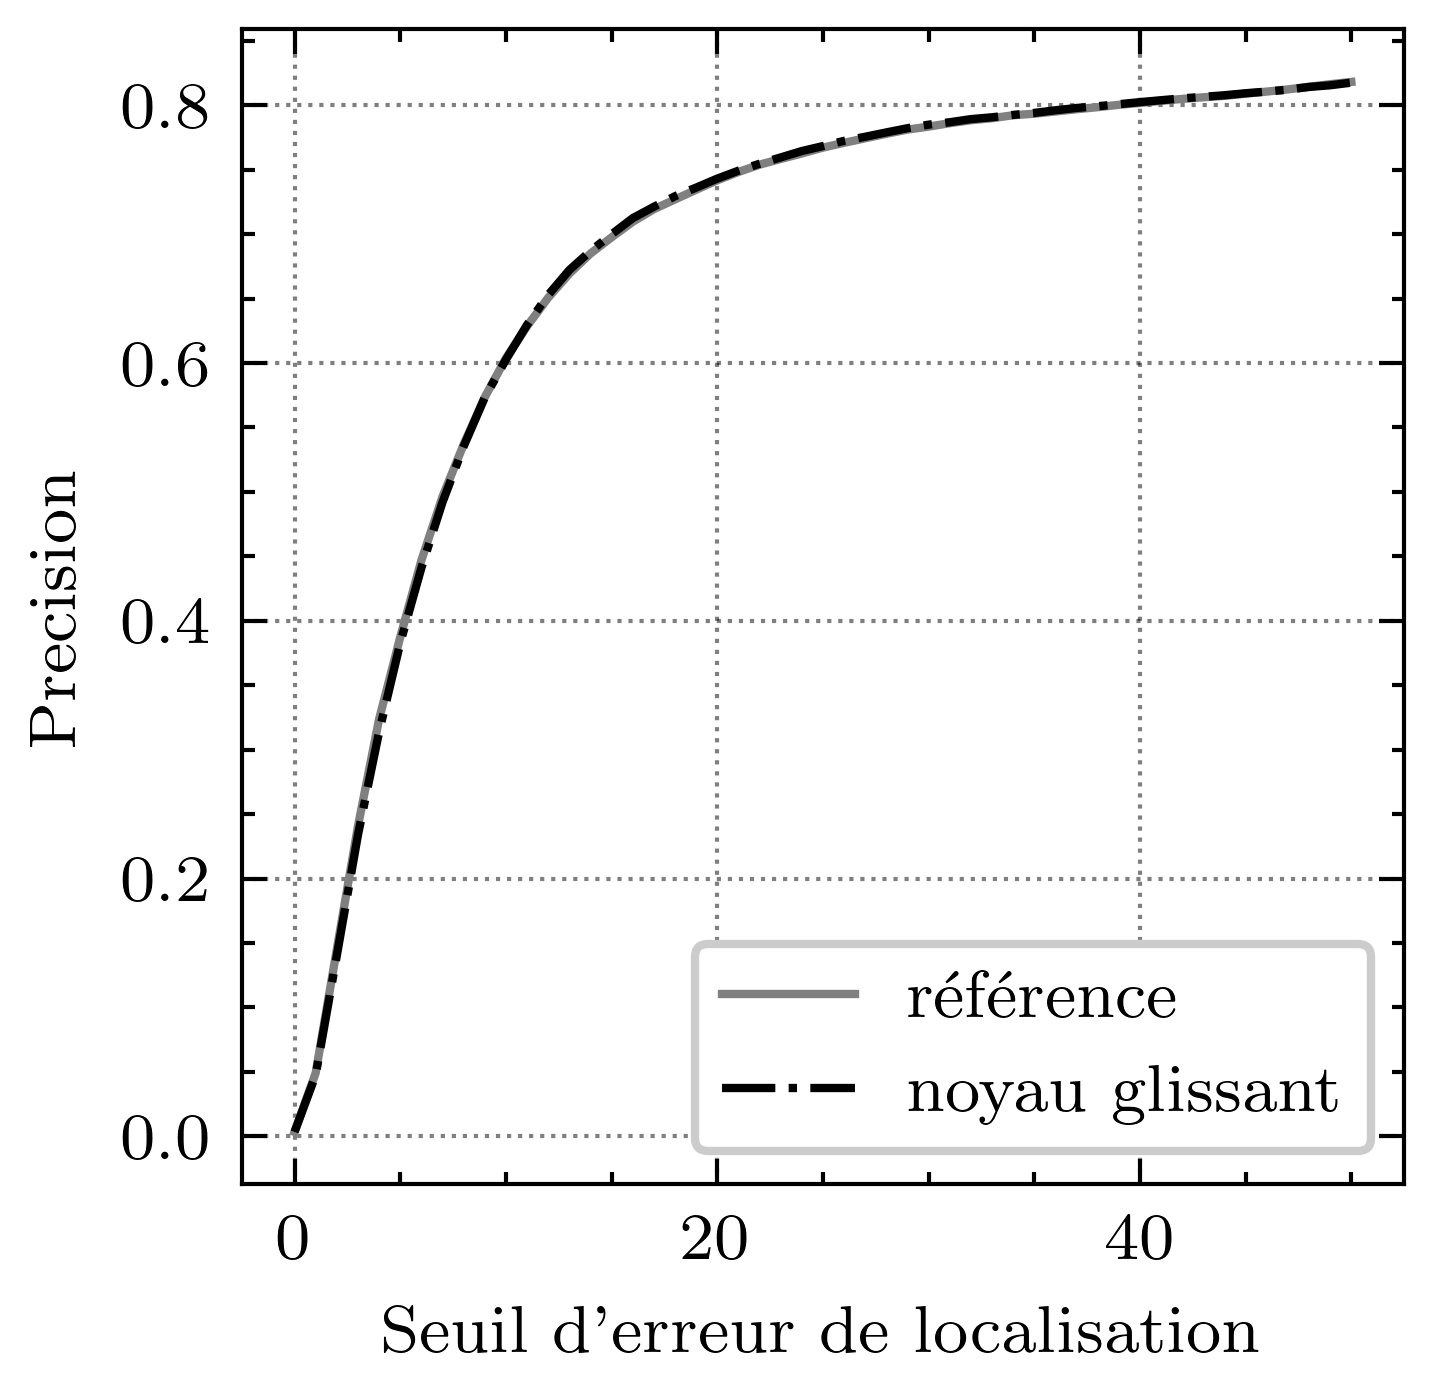
\includegraphics[width=125pt]{images/gamma/courbes_pre.png} 
  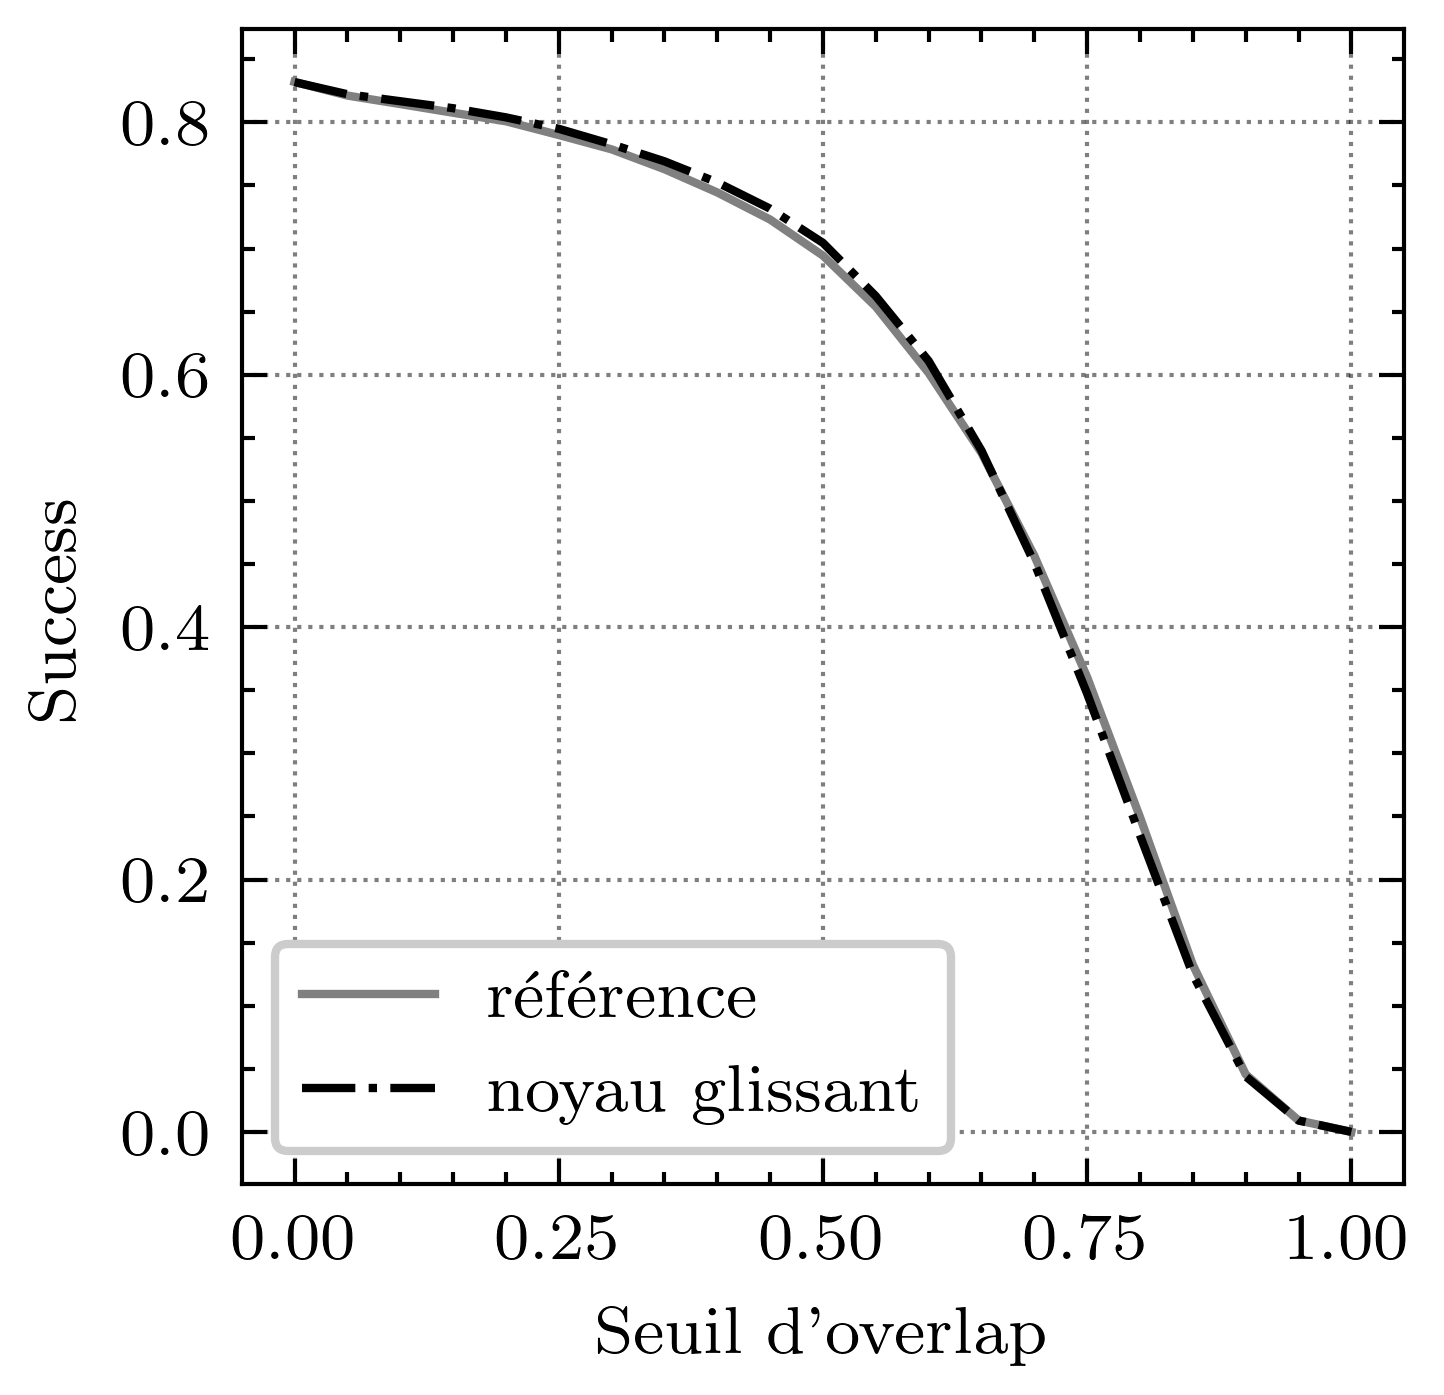
\includegraphics[width=125pt]{images/gamma/courbes_succ.png} 
  \caption{\textbf{Comparaison des performances de la méthode de référence et du noyau glissant.} Les performances globales sont proches, mais le taux de succès est amélioré par le noyau glissant.}
  \label{courbes_prec2}
  \end{figure}
  
  \begin{figure*}[!h]
  \centering
  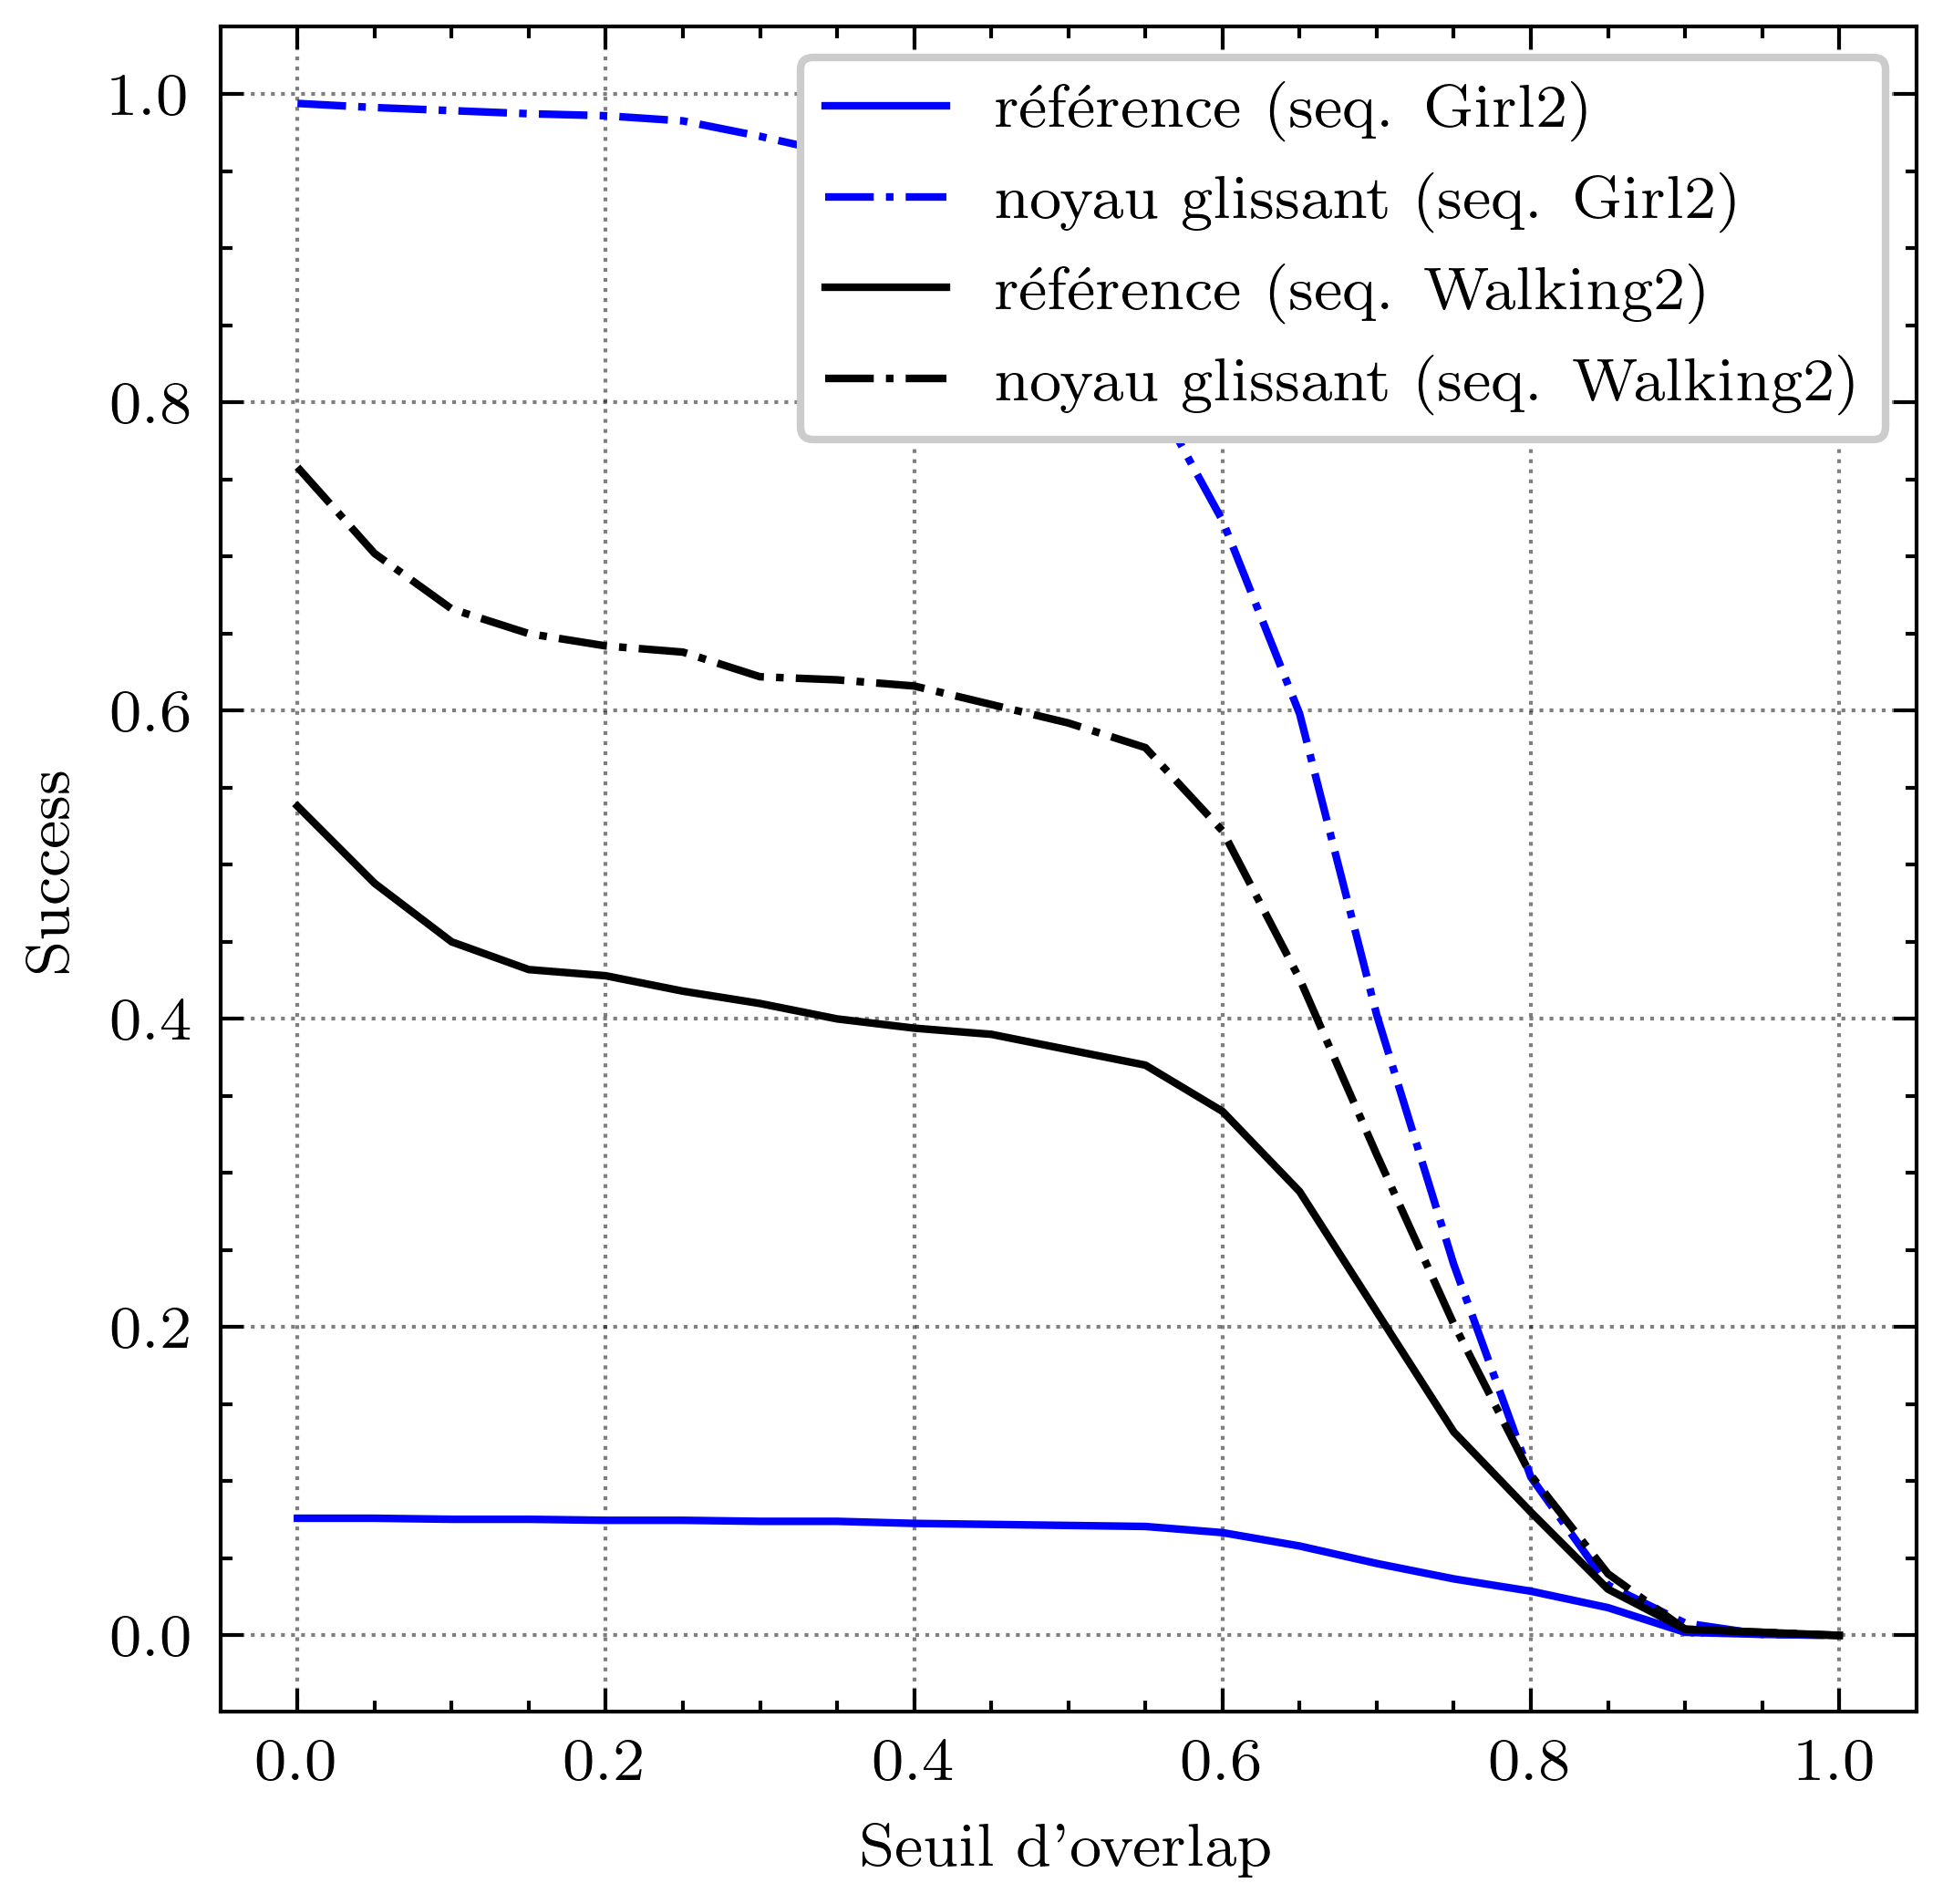
\includegraphics[width=150pt]{images/gamma/courbes_succ_mutli.png} 
  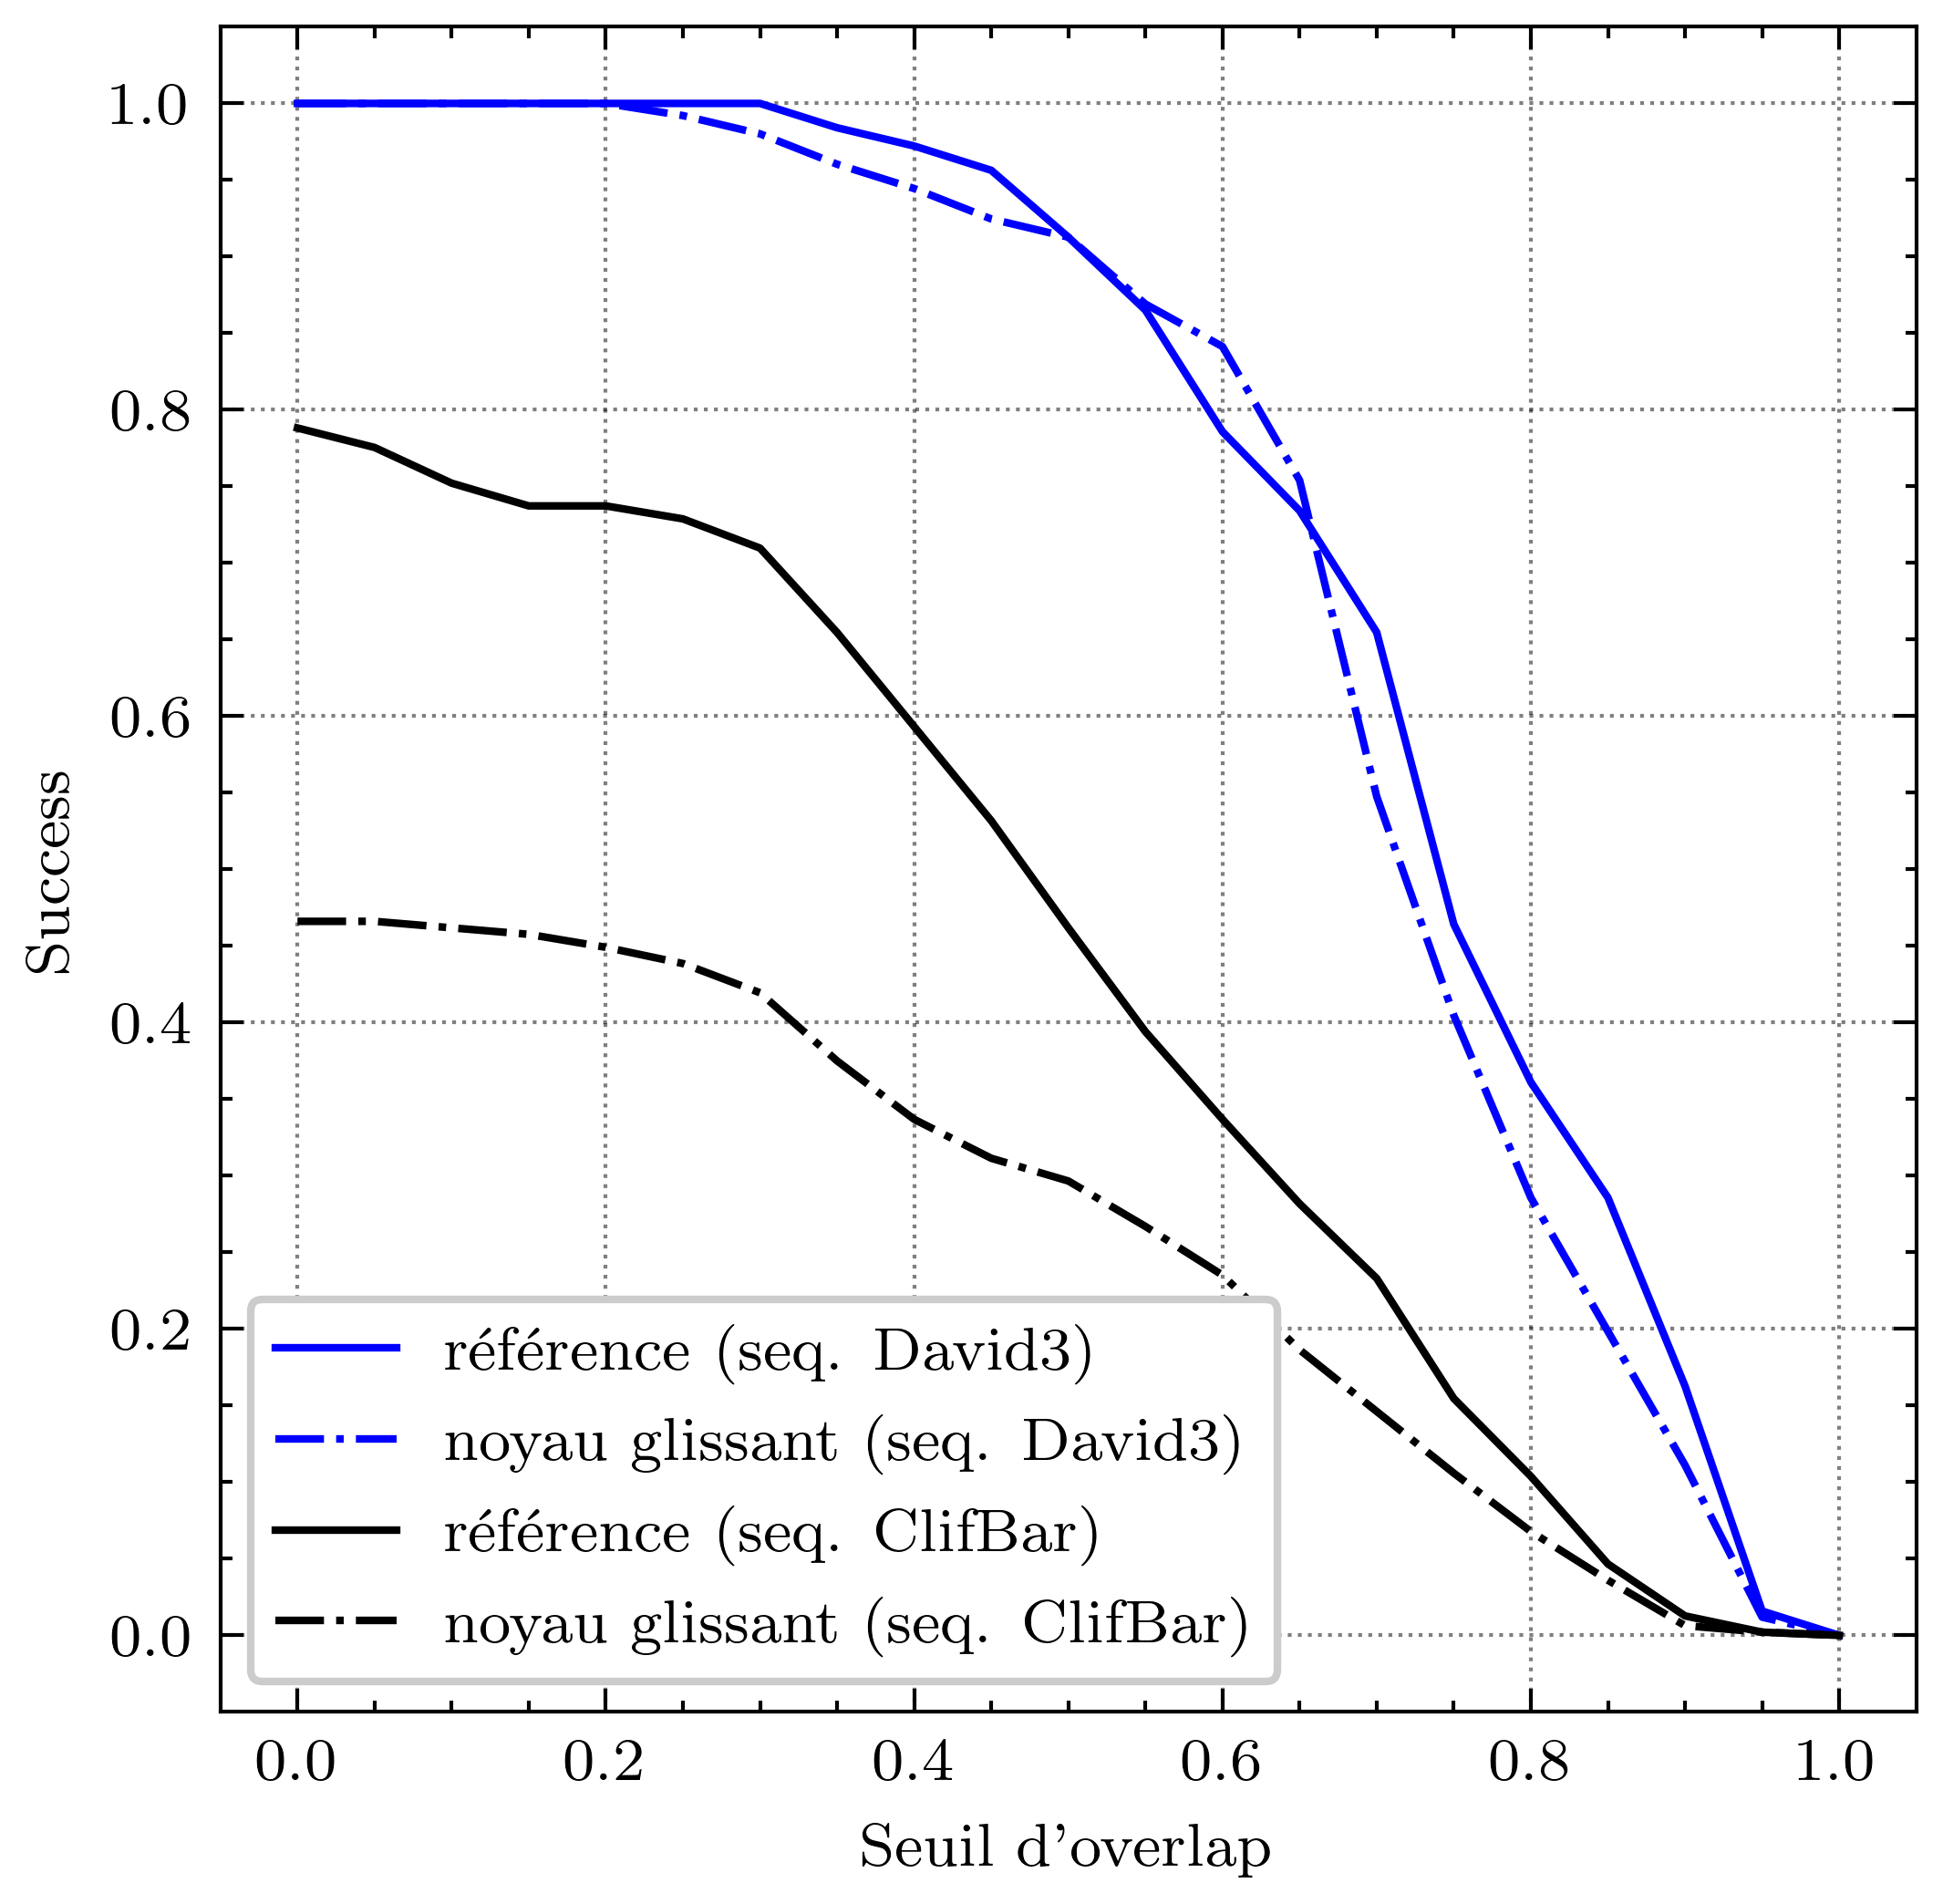
\includegraphics[width=150pt]{images/gamma/courbes_succ_mutli_bof.png} 
  \caption{\textbf{Comparaison des performances sur certaines séquences notables.} À gauche, les séquences \textit{Girl2} et \textit{Walking2} de OTB, pour lesquels l'amélioration est notable. À droite, les séquences \textit{David3} et \textit{ClifBar} de OTB, pour lesquels l'effet est négatif.}
  \label{courbes_prec3}
  \end{figure*}
 

Il est intéressant de noter que ces évolutions de performances ne sont pas équivalentes pour toutes les séquences de test. En particulier, la figure  \ref{courbes_prec3} montre des exemples de séquence où l'évolution de la performance est particulièrement bonne (\textit{Girl2} et \textit{Walking2} de OTB), et des exemples où le noyau glissant baisse significativement la performance  (\textit{David3} et \textit{ClifBar} de OTB). De tels différences poussent à étudier l'effet de la modification du modèle d'un point de vue qualitatif.
  




\subsubsection*{b. Analyse qualitative}


L'ajout du deuxième noyau défini dans \ref{noyau} apporte plusieurs avanatages qui se vérifient en explorant les résultats de l'expérimentation. Pour visualier ceci, nous avons marqué sur les images de sortie à la fois les prédictions faites par le suiveur de référence, les prédictions faites par le nouveau noyau, et enfin les prédictions faites par la moyenne pondérée des deux (la méthode finale). Quelques exemples sont donnés par la figure \ref{exemples_predictions}, où ces trois prédictions sont respectivement en rouge, en vert, et en bleu.

\begin{figure}[!h]
  \centering
  (a)
  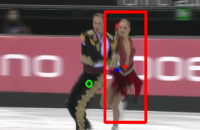
\includegraphics[width=120pt]{images/gamma/000469.png}\\
  (b)
  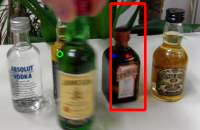
\includegraphics[width=120pt]{images/gamma/000726.png}\\
  (c)
  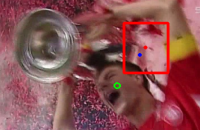
\includegraphics[width=120pt]{images/gamma/000038.png}\\
  (d)
  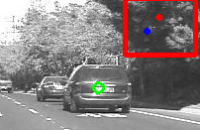
\includegraphics[width=120pt]{images/gamma/000414.png}\\
  \caption{\textbf{Effet qualitatif du noyau glissant sur le suivi.} Les points rouges sont les prédictions de référence. Les cercles verts sont les prédictions du noyau glissant. Les points bleus sont les moyennes pondérées des deux, pour $\beta=0.8$.}
  \label{exemples_predictions}
  \end{figure}

On y observe que le fait de garder en mémoire les images précédentes de la cible permet bien de gagner en robustesse vis à vis des changements d'apparence des objets. Par exemple, sur l'image (a) les danseurs tournent sur eux-même et la cible est le danseur. On observe que la changement de pose du danseur pousse le modèle de référence (en rouge) à prédire l'objet au niveau de la danseuse, alors que le noyau glissant (en vert) permet de rester sur le danseur.

De manière générale le noyau glissant assure une certaine inertie. Ceci est intuitif puisqu'il force le modèle à se concentrer sur les formes qu'il a déjà vu. Cet effet est très bénéfique pour le suivi puisque le modèle de référence a tendance à confondre des objets, que ce soit à cause d'une ressemblance, d'une obstruction, ou d'un flash (voir \textit{\nameref{echecs}}). L'effet d'inertie va empêcher la prédiction d'accrocher un autre objet qui n'est pas la cible, ce qui va laisser plus de chance au suiveur de revenir à la cible lors de la prochaine prédiction. C'est ce phénomène que montrent les images (b) à (d) de la figure  \ref{exemples_predictions}.

Ces remarques sont à fois des avantages et des inconvénients selon la situation. En effet, l'effet d'inertie peut limiter les performances du suiveur lorsque l'objet à suivre admet une vitesse relative très importante par rapport au repère de l'image (objet rapide ou instabilité de la caméra). De plus, bien que l'inertie limite le décrochage à la cible, elle limite aussi le réaccrochage. En d'autres termes, le suiveur sera plus robuste et fera moins d'erreur, mais dès lors que le suiveur décroche, les conséquences seront plus graves.

\subsubsection*{c. Travail futur}

Considérant les remarques du paragraphe précédent, on comprend qu'il est nécessaire d'ajuster l'importance du noyau glissant en fonction de la situation. Plus concrètement, il s'agira d'indexer le comportement du suiveur sur ses valeurs d'état interne, permettant de caractériser la situation. Esnuite, on peut adapter le comportement du suiveur à travers des hyper-paramètres (comme typiquement $\beta$ qui va permettre de plus ou moins prendre en compte l'effet du noyau glissant). Nous avons tenté cette amélioration en adaptant $\beta$ ainsi que $\gamma$ en fonction de :
\begin{itemize}
  \item la distance de la prédiction de référence à la prédiction précédente
  \item la distance de la prédiction du noyau glissant à la prédiction précédente
  \item la valeur maximale de la carte de corrélation de référence
  \item la valeur maximale de la carte de corrélation du noyau glissant
\end{itemize}
Le but étant de, pour ainsi dire, donner de l'importance au noyau glissant seulement lorsque celui-ci donne les signes d'une prédiction pertinente.

Nous avons implémenté cette méthode avec des règles définies à la main après observation qualitative des cas d'échecs. \textbf{Cette méthode n'a pas été concluante pour l'instant}. Cependant, cela ouvre la voie à une possiblité prometteuse : il est possible de modéliser la fonction qui donne la qualité de chacune des deux prédictions (de référence, et du noyau glissant) par un réseau de neurones qui prend en entrée les valeurs d'état du suiveur, ce qui permettrait \textbf{d'apprendre à donner de l'importance au noyau glissant}. Un tel réseau peut-être simple, et il pourrait même s'agir d'une simple combinaison linéaire des indicateurs s'il s'avère que l'expérience montre que c'est suffisant. Un point important est que la définition du noyau glissant ne contient que des dépendances simples et surtout différentiables. En conséquence, \textbf{il est possible de connaître l'erreur de prédiction en sortie de cette fonction}, ce qui permettrait d'entrainer efficacement ce réseau par rétropropagation. Ce travail demande du temps mais se présente comme la prochaine étape après ce rapport.

\section*{Conclusion}

Nous avons montré que la méthode de référence du siamFC, qui se base sur AlexNet, peut être légèrement améliorée à la fois en diminuant le nombre de couches et à la fois en ajoutant un noyau glissant. Ce noyau glissant a pour rôle de garder un historique des images de la cible, ce qui augmente la robustesse du suiveur. Nous avons montré que ce noyau glissant n'est utile que dans certaines situations. Par conséquence une prochaine amélioration consiste à prédire l'importance du noyau glissant à partir des états internes du suiveur. La structure générale de la méthode permet de calculer l'erreur sur cette estimation, ce qui permettrait un apprentissage efficace de l'importance du noyau, par rétropropagation.


{\small
\bibliographystyle{ieee}
\bibliography{rapport}
}

\clearpage
\onecolumn

\begin{appendices}

  \section{Quelques exemples de prédictions}
  \label{annexe_exemples}
  \subsection*{Exemples corrects}
  \begin{center}

    \hspace{1cm}

  \textbf{OTB} - \textit{Bolt}\\
  \hspace{1cm}\\
  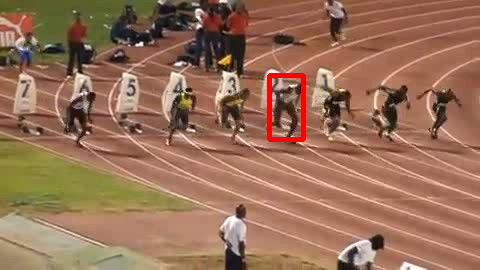
\includegraphics[width=85pt]{images/exemples/ok/bolt/000001.png}
  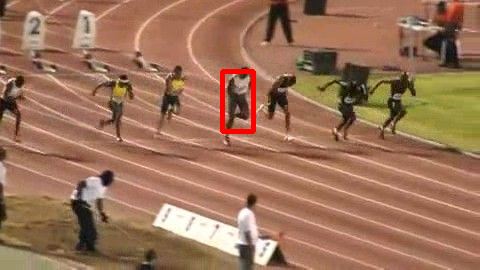
\includegraphics[width=85pt]{images/exemples/ok/bolt/000038.png}
  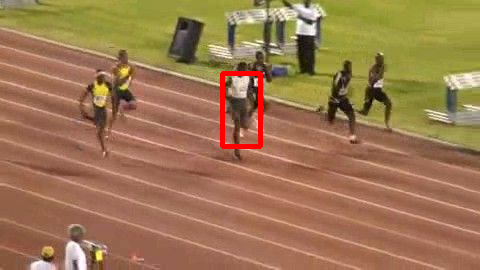
\includegraphics[width=85pt]{images/exemples/ok/bolt/000117.png}
  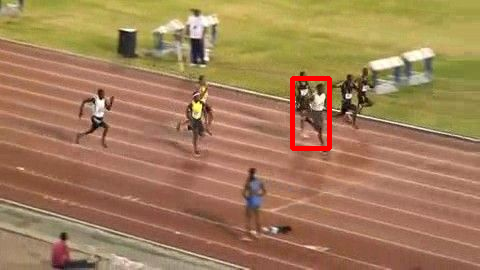
\includegraphics[width=85pt]{images/exemples/ok/bolt/000169.png}
  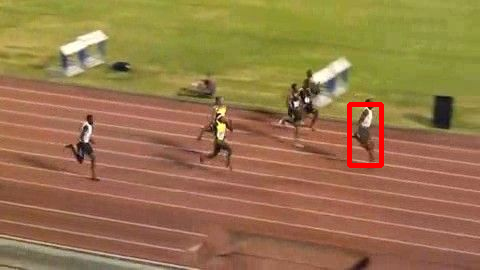
\includegraphics[width=85pt]{images/exemples/ok/bolt/000231.png}
  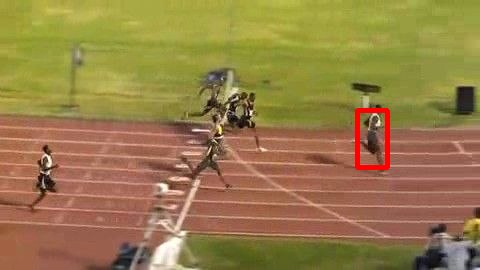
\includegraphics[width=85pt]{images/exemples/ok/bolt/000281.png}\\
  \hspace{1cm}\\
  \hspace{1cm}\\

  \textbf{OTB} - \textit{Car}\\
  \hspace{1cm}\\
  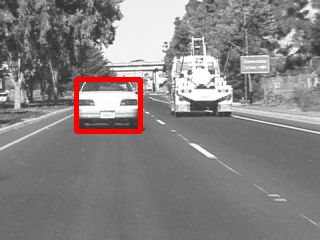
\includegraphics[width=85pt]{images/exemples/ok/car/000001.png}
  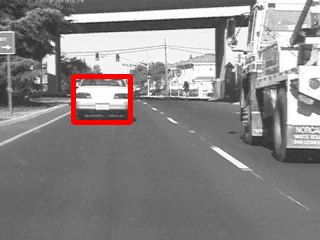
\includegraphics[width=85pt]{images/exemples/ok/car/000310.png}
  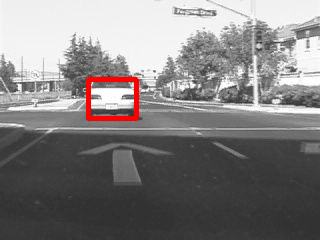
\includegraphics[width=85pt]{images/exemples/ok/car/000454.png}
  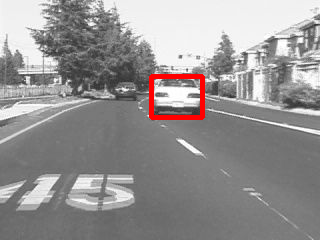
\includegraphics[width=85pt]{images/exemples/ok/car/000546.png}
  \includegraphics[width=85pt]{images/exemples/ok/car/000727.png}
  \includegraphics[width=85pt]{images/exemples/ok/car/000888.png}\\
  \hspace{1cm}\\
  \hspace{1cm}\\

  \textbf{OTB} - \textit{Dancer}\\
  \hspace{1cm}\\
  \includegraphics[width=85pt]{images/exemples/ok/dancer/000001.png}
  \includegraphics[width=85pt]{images/exemples/ok/dancer/000036.png}
  \includegraphics[width=85pt]{images/exemples/ok/dancer/000088.png}
  \includegraphics[width=85pt]{images/exemples/ok/dancer/000149.png}
  \includegraphics[width=85pt]{images/exemples/ok/dancer/000192.png}
  \includegraphics[width=85pt]{images/exemples/ok/dancer/000225.png}\\
  \hspace{1cm}\\
  \hspace{1cm}\\

  \textbf{OTB} - \textit{DragonBall}\\
  \hspace{1cm}\\
  \includegraphics[width=85pt]{images/exemples/ok/baby/000001.png}
  \includegraphics[width=85pt]{images/exemples/ok/baby/000020.png}
  \includegraphics[width=85pt]{images/exemples/ok/baby/000037.png}
  \includegraphics[width=85pt]{images/exemples/ok/baby/000053.png}
  \includegraphics[width=85pt]{images/exemples/ok/baby/000069.png}
  \includegraphics[width=85pt]{images/exemples/ok/baby/000100.png}\\
  \hspace{1cm}\\
  \hspace{1cm}\\

  \textbf{OTB} - \textit{Deer}\\
  \hspace{1cm}\\
  \includegraphics[width=85pt]{images/exemples/ok/deer/000001.png}
  \includegraphics[width=85pt]{images/exemples/ok/deer/000021.png}
  \includegraphics[width=85pt]{images/exemples/ok/deer/000028.png}
  \includegraphics[width=85pt]{images/exemples/ok/deer/000035.png}
  \includegraphics[width=85pt]{images/exemples/ok/deer/000059.png}
  \includegraphics[width=85pt]{images/exemples/ok/deer/000070.png}\\
  \hspace{1cm}\\
  \hspace{1cm}\\

  \textbf{OTB} - \textit{Football}\\
  \hspace{1cm}\\
  \includegraphics[width=85pt]{images/exemples/ok/foot/000001.png}
  \includegraphics[width=85pt]{images/exemples/ok/foot/000052.png}
  \includegraphics[width=85pt]{images/exemples/ok/foot/000103.png}
  \includegraphics[width=85pt]{images/exemples/ok/foot/000165.png}
  \includegraphics[width=85pt]{images/exemples/ok/foot/000263.png}
  \includegraphics[width=85pt]{images/exemples/ok/foot/000360.png}\\

  \end{center}
  \clearpage
  \subsection*{Exemples d'échecs}
  Les prédictions en vert sont correctes, les prédictions en rouge ne le sont pas.
  \begin{center}
    \hspace{1cm}

  \textbf{OTB} - \textit{Biker}\\
  \hspace{1cm}\\
  \includegraphics[width=82pt, cfbox=green 1pt 1pt]{images/exemples/bof/bike/000001.png}
  \includegraphics[width=82pt, cfbox=green 1pt 1pt]{images/exemples/bof/bike/000021.png}
  \includegraphics[width=82pt, cfbox=green 1pt 1pt]{images/exemples/bof/bike/000071.png}
  \includegraphics[width=82pt, cfbox=green 1pt 1pt]{images/exemples/bof/bike/000081.png}
  \includegraphics[width=82pt, cfbox=red 1pt 1pt]{images/exemples/bof/bike/000100.png}
  \includegraphics[width=82pt, cfbox=red 1pt 1pt]{images/exemples/bof/bike/000142.png}\\
  \hspace{1cm}\\
  \hspace{1cm}\\

  \textbf{OTB} - \textit{Box}\\
  \hspace{1cm}\\
  \includegraphics[width=82pt, cfbox=green 1pt 1pt]{images/exemples/bof/box/000001.png}
  \includegraphics[width=82pt, cfbox=green 1pt 1pt]{images/exemples/bof/box/000119.png}
  \includegraphics[width=82pt, cfbox=red 1pt 1pt]{images/exemples/bof/box/000311.png}
  \includegraphics[width=82pt, cfbox=green 1pt 1pt]{images/exemples/bof/box/000567.png}
  \includegraphics[width=82pt, cfbox=green 1pt 1pt]{images/exemples/bof/box/000839.png}
  \includegraphics[width=82pt, cfbox=green 1pt 1pt]{images/exemples/bof/box/001127.png}\\
  \hspace{1cm}\\
  \hspace{1cm}\\

  \textbf{OTB} - \textit{Coupon}\\
  \hspace{1cm}\\
  \includegraphics[width=82pt, cfbox=green 1pt 1pt]{images/exemples/bof/coupon/000001.png}
  \includegraphics[width=82pt, cfbox=green 1pt 1pt]{images/exemples/bof/coupon/000054.png}
  \includegraphics[width=82pt, cfbox=green 1pt 1pt]{images/exemples/bof/coupon/000104.png}
  \includegraphics[width=82pt, cfbox=red 1pt 1pt]{images/exemples/bof/coupon/000133.png}
  \includegraphics[width=82pt, cfbox=red 1pt 1pt]{images/exemples/bof/coupon/000215.png}
  \includegraphics[width=82pt, cfbox=red 1pt 1pt]{images/exemples/bof/coupon/000322.png}\\
  \hspace{1cm}\\
  \hspace{1cm}\\

  \textbf{OTB} - \textit{Human3}\\
  \hspace{1cm}\\
  \includegraphics[width=82pt, cfbox=green 1pt 1pt]{images/exemples/bof/human/000001.png}
  \includegraphics[width=82pt, cfbox=green 1pt 1pt]{images/exemples/bof/human/000008.png}
  \includegraphics[width=82pt, cfbox=red 1pt 1pt]{images/exemples/bof/human/000035.png}
  \includegraphics[width=82pt, cfbox=red 1pt 1pt]{images/exemples/bof/human/000054.png}
  \includegraphics[width=82pt, cfbox=red 1pt 1pt]{images/exemples/bof/human/000086.png}
  \includegraphics[width=82pt, cfbox=red 1pt 1pt]{images/exemples/bof/human/000117.png}\\
   \hspace{1cm}\\
  \hspace{1cm}\\
  
  
 \textbf{OTB} - \textit{Skiing}\\
  \hspace{1cm}\\
  \includegraphics[width=82pt, cfbox=green 1pt 1pt]{images/exemples/bof/skiing/000001.png}
  \includegraphics[width=82pt, cfbox=green 1pt 1pt]{images/exemples/bof/skiing/000008.png}
  \includegraphics[width=82pt, cfbox=red 1pt 1pt]{images/exemples/bof/skiing/000024.png}
  \includegraphics[width=82pt, cfbox=red 1pt 1pt]{images/exemples/bof/skiing/000040.png}
  \includegraphics[width=82pt, cfbox=red 1pt 1pt]{images/exemples/bof/skiing/000056.png}
  \includegraphics[width=82pt, cfbox=red 1pt 1pt]{images/exemples/bof/skiing/000072.png}\\
  
  \end{center} 
  \clearpage
  \section{Les différentes architectures testées}
  \label{annexe_archis}
  
  
  	\textit{Les matrices d'entrée (images à 3 canaux) ne sont pas représentées à l'échelle pour des raisons de lisibilité.}\\
  	\hspace{1cm}\\

    Architecture à 2 couches.
    \begin{center}
    \includegraphics[height=160pt]{images/archis/convnet_cnn2.png}
    \end{center}
    \hspace{1cm}\\
    \hspace{1cm}\\

    Architecture à 3 couches.
    \begin{center}
    \includegraphics[height=160pt]{images/archis/convnet_cnn3.png}
    \end{center}
    \hspace{1cm}\\
    \hspace{1cm}\\
  
    Architecture à 4 couches.
    \begin{center}
    \includegraphics[height=160pt]{images/archis/convnet_cnn4.png}
    \end{center}
    \clearpage

    Architecture à 5 couches (modèle de référence \cite{siamfc}).
    \begin{center}
    \includegraphics[height=160pt]{images/archis/convnet_cnn5.png}
    \end{center}
    \hspace{1cm}\\
    \hspace{1cm}\\

    Architecture à 6 couches.
    \begin{center}
    \includegraphics[height=160pt]{images/archis/convnet_cnn6.png}
    \end{center}
    \hspace{1cm}\\
    \hspace{1cm}\\

    Architecture à 7 couches.
    \begin{center}
    \includegraphics[height=160pt]{images/archis/convnet_cnn7.png}
    \end{center} 




  \end{appendices}

\end{document}
